\documentclass[../main]{subfiles}
\ifSubfilesClassLoaded{
    \dominitoc
    \tableofcontentsfile
	\pagenumbering{arabic}
    \setcounter{page}{1}
	\setcounter{chapter}{6}
	\addbibresource{../Biblio/biblio.bib}
}{}

\begin{document}
\graphicspath{{../06b-Analyse-2D}, {06b-Analyse-2D}}

\chapter{Extension des mécanismes d'auto-organisation aux cartes en deux dimensions}\label{chap:analyse2D}

\minitoc

\section{Introduction}

Dans les chapitres précédents, nous avons étudié les propriétés d'organisation de cartes en une dimension d'une architecture de cartes CxSOM.
L'étude des cartes en une dimension nous offrait un cadre de représentation facile pour la mise en valeur des mécanismes d'organisation et d'apprentissage des relations entre les entrées.
Cependant, les cartes auto-organisatrices généralement utilisées en pratique sont des cartes en deux dimensions. 
Elles apportent une meilleure qualité de quantification vectorielle sur des données de plus grande dimension que les cartes 1D, tout en restant assez peu coûteuses en nombre de n\oe{}uds.
Dans les SOM classiques, le passage de cartes 1D à des cartes 2D fait apparaître des mécanismes d'organisation plus variés grâce à la dimension supplémentaire, mais pose également des problèment supplémentaire en terme de convergence des poids.
Nous cherchons ainsi à vérifier dans ce chapitre si les mécanismes d'organisation observés sur des architectures de cartes en une dimension s'observent également sur des cartes en deux dimensions et si la 2D pose des limites.
Le modèle CxSOM tel que présenté au chapitre~\ref{chap:modele} est adapté à des cartes de dimension et de voisinage quelconque. 
Les expériences présentées dans ce chapitre ne nécessitent pas d'adaptation spécifique de l'algorithme.

Nous avons étudié des architectures de deux et trois cartes 1D~; nous nous intéresserons dans ce chapitre à des architectures de deux et trois cartes 2D.
Le but est de vérifier si les mécanismes observés dans ces architectures de cartes 1D sont observés en 2D. 
Nous observerons les comportements suivants, qui, nous l'avons vu, marquent l'apprentissage des entrées et de leurs relations dans des architectures de cartes 1D~:
\begin{itemize}
	\item Les poids externes de chaque carte de l'architecture permettent une bonne quantification vectorielle de leur entrée externe.
	\item Les poids contextuels définissent des zones et se déplient en formant des sous-cartes sur des zones de la carte.
	\item Les BMUs d'une carte encodent à la fois l'entrée externe et la valeur du modèle $U$ grâce aux zones de poids contextuels, formant deux échelles d'indices.
	\item Une carte ne recevant pas d'entrée externe est capable de générer une bonne prédiction de la modalité manquante dans l'architecture.
\end{itemize}

Nous vérifierons également que la relaxation converge correctement sur des cartes en deux dimensions.
Les exemples que nous étudions dans ce chapitre nous permettront d'identifier des limites et perspectives pour le passage des cartes 1D à 2D dans des architectures de cartes.

\section{Présentation de l'expérience}

\subsection{Architecture de carte 2D}

L'architecture de cartes en deux dimensions est construite sur le même principe qu'une architecture de cartes 1D, le modèle présenté au chapitre \ref{chap:modele} étant valable pour n'importe quelle dimension de carte.

Les n\oe{}uds d'une carte sont positionnées sur une grille carrée de taille $100 \times 100$ et indexés entre 0 et 1 sur chaque dimension. Nous notons cet index $\mathbf{p}\m{i} = (p\m{i}|_x, p\m{i}|_y)$ sur les figures. 
Chaque carte possède donc une couche de poids externes $\w\ext \in [0,1]^2$ et une couche de poids contextuels $\w_c \in [0,1]^2$.
L'entrée contextuelle correspond à la position du BMU de l'autre carte. Il s'agit des positions 2D $\mathbf{p}\m{2}$ pour la carte $M\m{1}$ et $\mathbf{p\m{1}}$ pour la carte $M\m{2}$. 


Les activités $a_e$ et $a_c$ sont calculées par une activation gaussienne~:
$$a_e(\inpx,\mathbf{p}) = \exp(\frac{||\inpx - \w_e(\mathbf{p}) ||^2}{2\sigma^2})$$
de même pour $a_c$.
La norme utilisée est ici la norme euclidienne, que ce soit dans l'espace d'entrée et dans l'espace des positions de la carte. Les fonctions de voisinage sont également définies à partir de la norme euclidienne dans l'espace des positions d'une carte.

La notion d'organisation dans une carte 2D est plus difficile à formuler que dans une carte en une dimension.
Par exemple, la topologie intuitive d'une carte "organisée" sur le carré $[0,1]^2$ est que les quatre coins de la carte viennent se placer dans les coins du carré. Cependant, les mécanismes d'organisation peuvent conduire à une carte tordue en son milieu, par exemple en \label{fig:torsion}. 
Cette organisation avec un point de torsion respecte la continuité des poids au sens des cartes auto-organisatrices~: deux poids proches dans la carte correspondent à des entrées proches, il s'agit d'une configuration stable de poids, mais ce n'est pas forcément la topographie représentant le mieux l'espace d'entrée. 
Dans une architecture CxSOM, cela pourrait poser un problème pour l'utilisation de la position du BMU en tant que représentation de l'entrée~: deux entrées proches peuvent avoir leur BMU de chaque côté de la carte.
%Des mesures d'organisation existent sur des cartes en deux dimensions \cite{Polani2001MeasuresFT}.

\begin{figure}
	\centering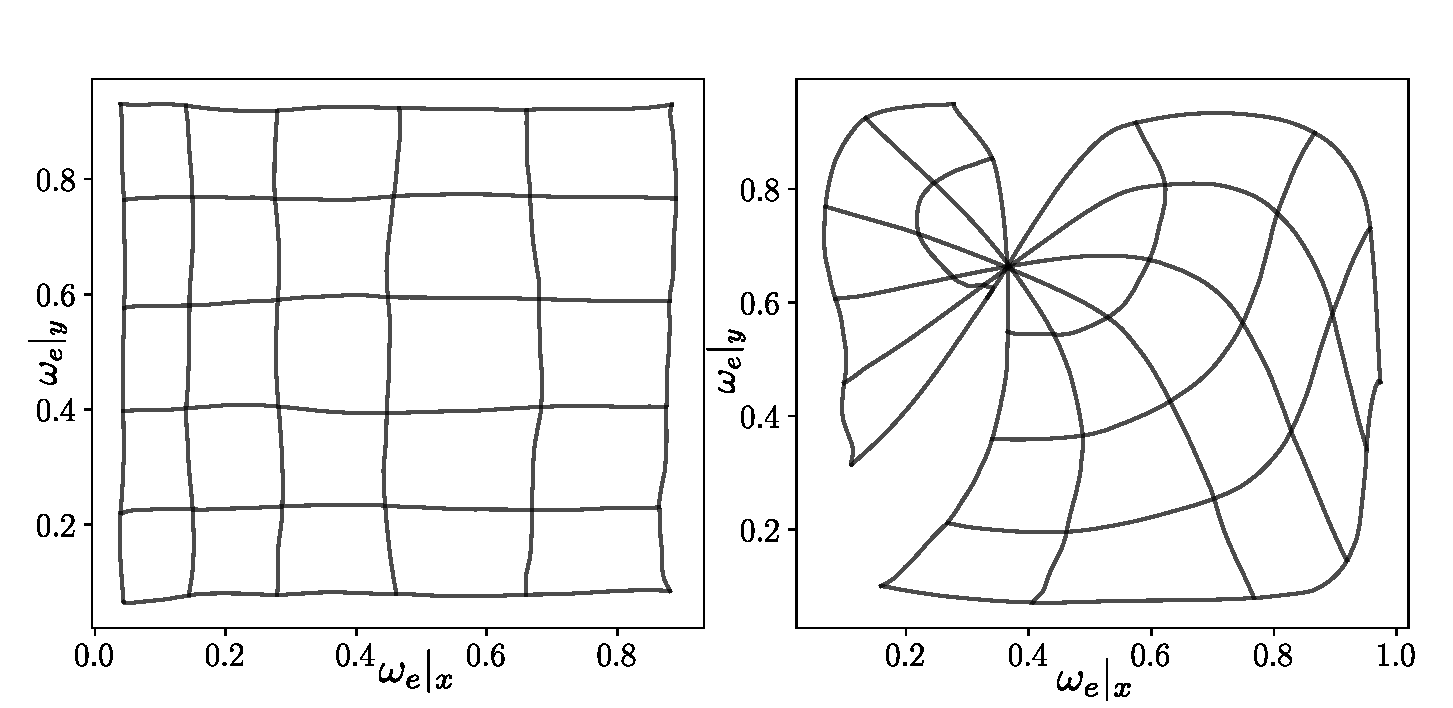
\includegraphics[width=0.7\textwidth]{grid_torsion.pdf}
	\caption{Exemples d'organisation de cartes classiques sur des entrées présentées dans $[0,1]^2$. 
	La carte de gauche est \og bien dépliée \fg{}~: deux entrées proches sont représentées par des BMUs proches. 
	Au contraire, la disposition de droite présente un point de torsion. Cette disposition peut évoluer vers une carte bien dépliée ou vers un état stable qui présente encore un point de torsion, en fonction des paramètres d'apprentissage. Dans ce dernier cas, la carte est toujours organisée et a appris les entrées, mais cette organisation est moins souhaitable que dans le cas de gauche. \label{fig:torsion}
	}
\end{figure}
De plus, l'organisation et la convergence des poids externes n'est pas assurée en 2D lorsque l'on prend un rayon de voisinage constant, ce qui est le cas dans CxSOM.
Des travaux ont prouvé la convergence des SOM en une dimension, mais seulement partiellement pour les cartes en deux dimensions, même lorsque les paramètres d'apprentissage décroissants \cite{flanagan_self-organisation_1996}. 
En pratique, la convergence des poids des SOMs en deux dimensions est bien observée avec un rayon de voisinage décroissant, mais aucun travail à notre connaissance n'a étudié la convergence de SOMs 2D lorsque les rayons restent constants. La convergence des poids des cartes est donc une propriété à vérifier expérimentalement en deux dimensions.

Dans les expériences de ce chapitre, nous avons choisi de favoriser le bon dépliement des poids externes en laissant les poids externes s'organiser seuls sur 1000 itérations à partir des activités externes, sans prendre en compte les poids contextuels. Cette pré-organisation est réalisée en prenant un grand rayon de voisinage $r_e = 0.5$. 
Ce grand rayon permet d'éviter les zones de torsion dans la carte et pré-répartit les poids externes sur les entrées externes. Après cette étape préalable, nous réduisons le rayon externe à $r_e = 0.2$ et effectuons l'apprentissage des poids externes et contextuels comme décrit dans le modèle CxSOM. Les poids externes affinent alors leur apprentissage. 
Cette étape ne change pas fondamentalement le comportement des cartes, étant donné que la différence d'échelle entre les rayons externes et contextuels permettait déjà aux poids externes de s'organiser plus rapidement que les poids contextuels.

% Les cartes 2D utilisées dans ce chapitre possèdent $10000$ n\oe{}uds (grille $100 \times 100$). Les cartes ont en effet besoin de  n\oe{}uds sur chaque dimension pour pouvoir avoir la place de former en zones.

\subsection{Modèles d'entrées}

Jusqu'à présent, les modalités observées étaient chacune en une dimension et $U$, la variable latente également une variable 1D.
Afin de complexifier la structure des entrées, nous choisissons dans ce chapitre d'utiliser des entrées dont chaque modalité est en deux dimensions, et dont le modèle latent $U$ est également 2D.
Nous analyserons des architectures de deux et trois cartes, ainsi nous choisissons des modèles d'entrées de dimension totale 4 et 6.

Comme dans le cas du cercle, nous choisissons un premier modèle d'entrée dans lequel une même valeur de $\inpx\m{1}$ corresponde à deux valeurs de $U$, afin de voir si les cartes sont capables de différencier leur BMU en fonction de $U$.
Ce modèle en version 4D est présenté en figure~\ref{fig:sphere_inputs}. La variable $U$ est une valeur 2D paramétrant des points placés sur une sphère 3D. 
Les deux dimensions de $U$ sont les angles paramétrant la représentation polaire de la sphère, $\theta$ et $\phi$ que nous prenons ici normalisés entre $0$ et $1$.
Pour générer les entrées, nous tirons $U$ dans $[0,1]^2$, ce qui génère un point sur la sphère.
Nous changeons ensuite de repère par une rotation en 4D afin que les coordonnées du point soient distribuées sur les 4 axes de l'espace 4D.
Cette représentation en 4D des points de la sphère permet de définir deux modalités en deux dimensions $\inpx\m{1}$ et $\inpx\m{2}$. Sur la figure, les points à chaque étape sont colorés par rapport à la valeur de $U$ représentée en figure de gauche.
Les paires $\inpx\m{1}, \inpx\m{2}$ correspondant à un même point sont présentées lors de la même itération à l'architecture.
Plusieurs valeurs de $U$ correspondent à une même valeur de $\inpx\m{1}$, ce qui est marqué par l'existence de plusieurs couleurs de points à une même position. C'est également le cas pour $\inpx\m{2}$.
Nous sommes donc dans un cas similaire aux tracés en une dimension, et nous chercherons à vérifier si les cartes $M\m{1}$ et $M\m{2}$ apprennent à différencier les valeurs de $U$ par la position de leur BMU.

\begin{figure}
	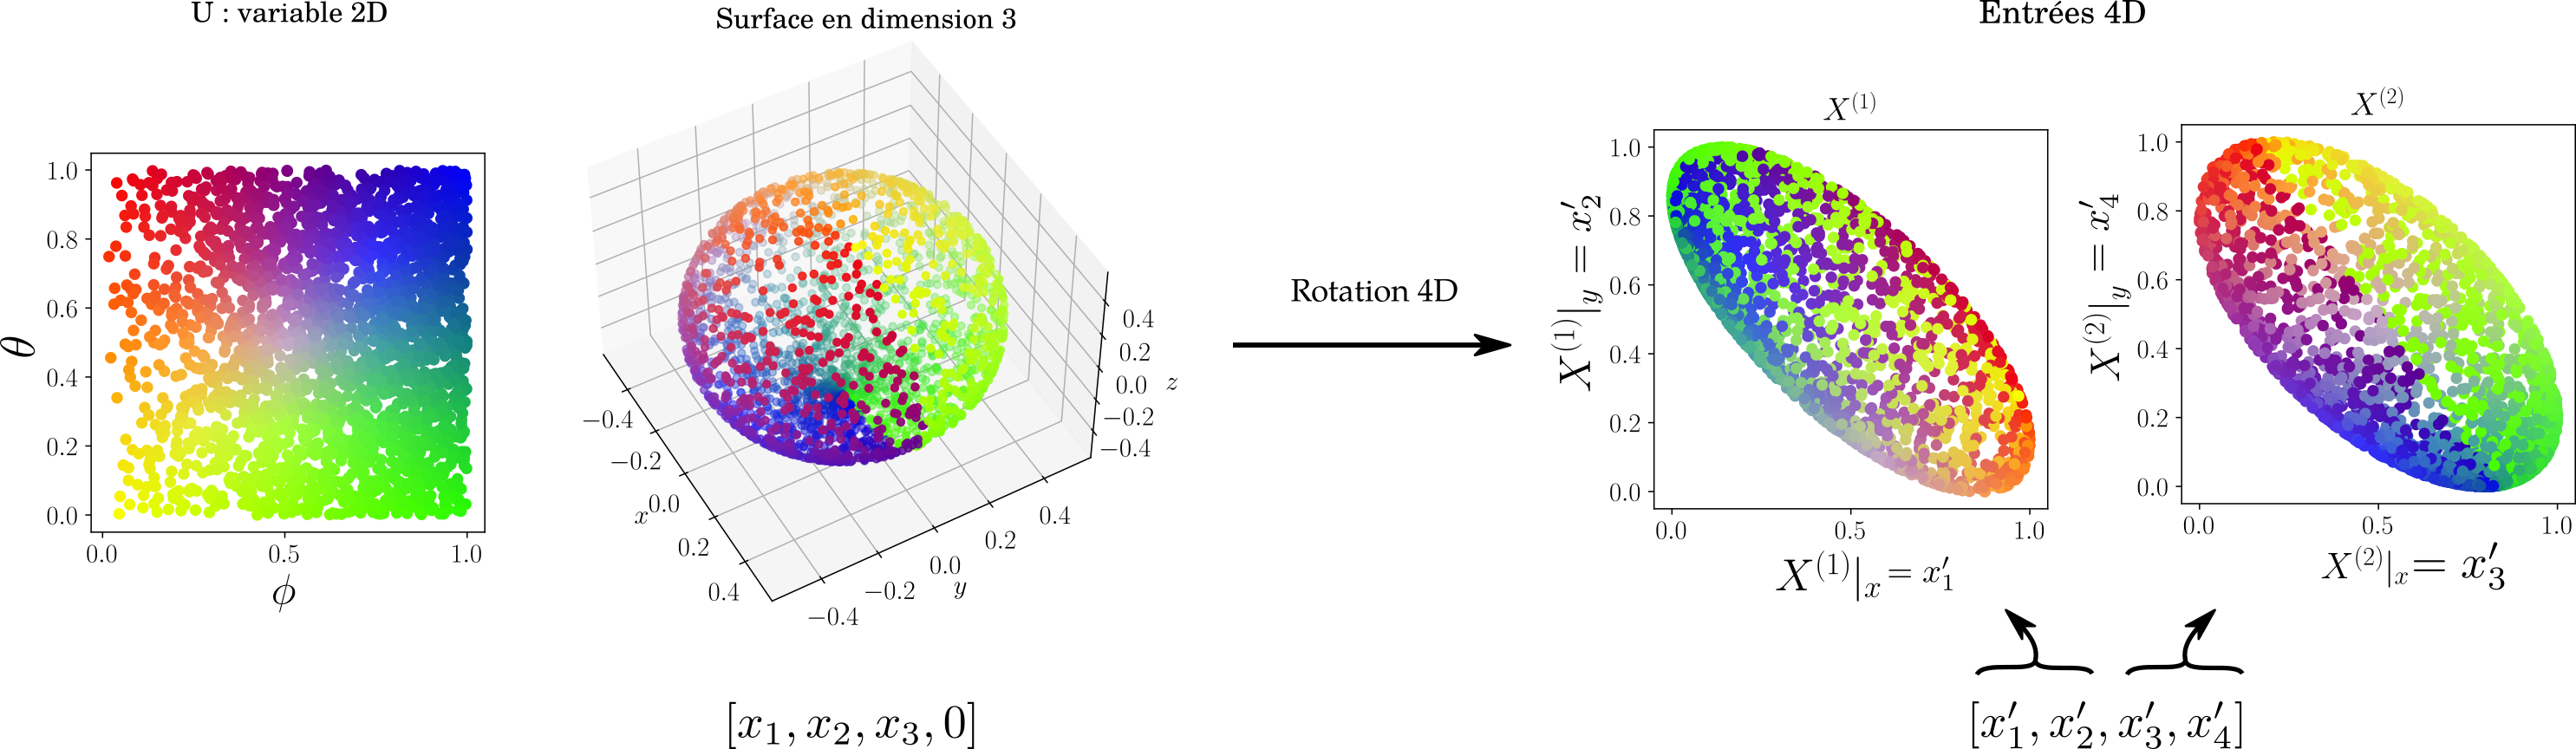
\includegraphics[width=\textwidth]{sphere_inputs_colormap.png}
	\caption{Transformation de la sphère 3D paramétrée par $U$ vers un espace 4D. La rotation permet de répartir les coordonnées des points sur les quatre dimensions sans modifier la structure des entrées. Les modalités considérées sont des valeurs 2D $\inpx\m{1}$ et $\inpx\m{2}$.
	La couleur de chaque point des figures fait référence à la valeur de $U$ correspondante, dont la disposition est présentée figure de gauche. Plusieurs valeurs de $U$ différentes permettent de générer une même valeur de $\inpx\m{1}$. Par exemple, $\inpx\m{1} = (0.5, 0.7)$ correspond à $U$ autour de $(0.6,0.3)$ (vert) ou $U$ autour de $ (0.6,0.8)$ (violet).
	\label{fig:sphere_inputs}}
\end{figure}

Nous utiliserons comme second modèle d'entrées 4D des points placés dans l'hypercube de dimension 4 $[0,1]^4$. Dans cette configuration, les deux modalités 2D $\inpx\m{1}$ et $\inpx\m{2}$ sont indépendantes, rappelant la configuration des entrées prises dans le patch $[0,1]^2$ pour des modalités 1D. L'étude de configuration d'entrées indépendantes permet d'évaluer les mécanismes d'organisation des cartes dans un cas limite.
Nous comparerons l'organisation des cartes 2D sur cet hypercube à celle que nous avions obtenue en 1D sur le patch $[0,1]^2$. 


Nous utiliserons enfin l'architecture de trois cartes sur un modèle d'entrées en six dimensions construit à partir d'une sphère 3D selon la méthode présentée plus haut. 
Les modalités sont chacune en deux dimensions et $U$ est une variable 2D.
Dans cette configuration, la connaissance de deux modalités sur trois détermine la troisième valeur, nous permettant d'observer la capacité de prédiction d'une architecture de cartes 2D.

\subsection{Expériences}

Ce chapitre est une série d'observations réalisées sur les architectures de cartes 2D cherchant à généraliser les comportements observés au long des chapitres précédents sur les architectures de cartes 1D.
Nous utilisons la même méthode expérimentale qu'en 1D, en adaptant les tracés déjà utilisés au cas des cartes en deux dimensions.

Sur une architecture de deux cartes apprenant sur les entrées disposées en sphères, nous observerons d'abord la disposition des poids externes et contextuels après apprentissage. Nous verrons que les poids externes se disposent comme les poids d'une carte auto-organisatrices classiques et que les poids contextuels forment des zones similaires à celles observées sur les cartes 1D au paragraphe~\ref{par:orga2D}.
Au paragraphe ~\ref{par:U_bmu2D}, nous tracerons la disposition des valeurs de $U$ selon la position du BMU. Cette représentation nous permettra de faire apparaître les zones mortes et de vérifier si les positions du BMU se séparent selon $U$. Nous utiliserons le ratio de corrélation présenté au chapitre \ref{chap:indicateur} pour évaluer cette organisation.
En 1D, le rayon $r_c$ détermine l'organisation en zones. Nous chercherons à traduire cette propriété en 2D et comparerons l'organisation obtenue pour différents rayons de voisinage contextuels au paragraphe \ref{par:params2D}.
Nous observerons ensuite la convergence de la relaxation sur ces expériences au paragraphe \ref{par:conv2D}.

En \ref{par:cub2D}, nous observerons la disposition des poids externes et contextuels après apprentissage d'entrées positionnées dans l'hypercube $[0,1]^4$, en effectuant un parallèle à l'expérience sur le patch $[0,1]^2$ avec une architecture de deux cartes 1D. Cette expérience permet de se placer dans un cas limite d'entrées et observer seulement le comportement induit par les règles de calcul de la carte.



Nous étudierons enfin au paragraphe \ref{par:pred2D} un cas d'architecture de trois cartes 2D, apprenant sur le modèle d'entrée en sphère 3D pivotée en six dimensions. Nous verrons si l'organisation observée sur l'architecture de deux cartes se généralise à trois cartes et si les cartes sont capables d'effectuer une tâche de prédiction d'entrée manquante.

\section{Résultats}

\subsection{Organisation des poids des cartes sur les entrées en sphère \label{par:orga2D}}

Nous étudions d'abord l'organisation des cartes sur les données prises sur la sphère 3D pivotée dans un espace en 4D décrite en figure \ref{fig:sphere_inputs}. Nous prendrons dans cette première expérience les rayons de voisinage à $r_c = 0.02$ et $r_e = 0.2$. 
Nous nous intéressons en premier lieu à l'organisation des poids externes et contextuels des cartes. Sur des cartes 1D, nous avons observé que les poids externes s'organisent comme une carte classique, tandis que les poids contextuels forment des zones.
La figure~\ref{fig:2som_s_002_wc}, en haut, présente la disposition des poids externes et contextuels de l'architecture de deux cartes après apprentissage.
En haut, nous représentons les poids externes dans l'espace des entrées~: un n\oe{}ud de la carte est positionné en $\w_e(\mathbf{p})$ qui est une position 2D.
La figure montre que chaque carte représente ses entrées externes de la même façon qu'une carte classique, comportement que nous attendions du modèle CxSOM~: les poids externes de chaque carte s'étendent sur le disque dans lequel sont tirées leurs entrées externes. Notons au passage que la quantification vectorielle est bien réalisée sur les entrées externes.
En bas, nous représentons les poids contextuels de la carte sous forme de carte de coloration. Un pixel positionné en position $\mathbf{p}$ est coloré selon la valeur de son poids $\w_c(\mathbf{p})$, une valeur en deux dimensions.
Ces tracés font apparaître des motifs alternés dans chaque carte qui rappellent les motifs présents en une dimension. Le comportement de zones observé en 1D se retrouve donc sur cet exemple de carte 2D.
Une première différence avec les cartes en une dimension est la forme des zones. On a en effet un degré de liberté supplémentaire pour l'organisation.
Comme en 1D, les zones sont de taille équivalentes réparties sur toute la surface de la carte. L'organisation des poids contextuels en zones est donc similaire entre 1D à 2D.

\begin{figure}[ht!]
	\begin{minipage}{\textwidth}
	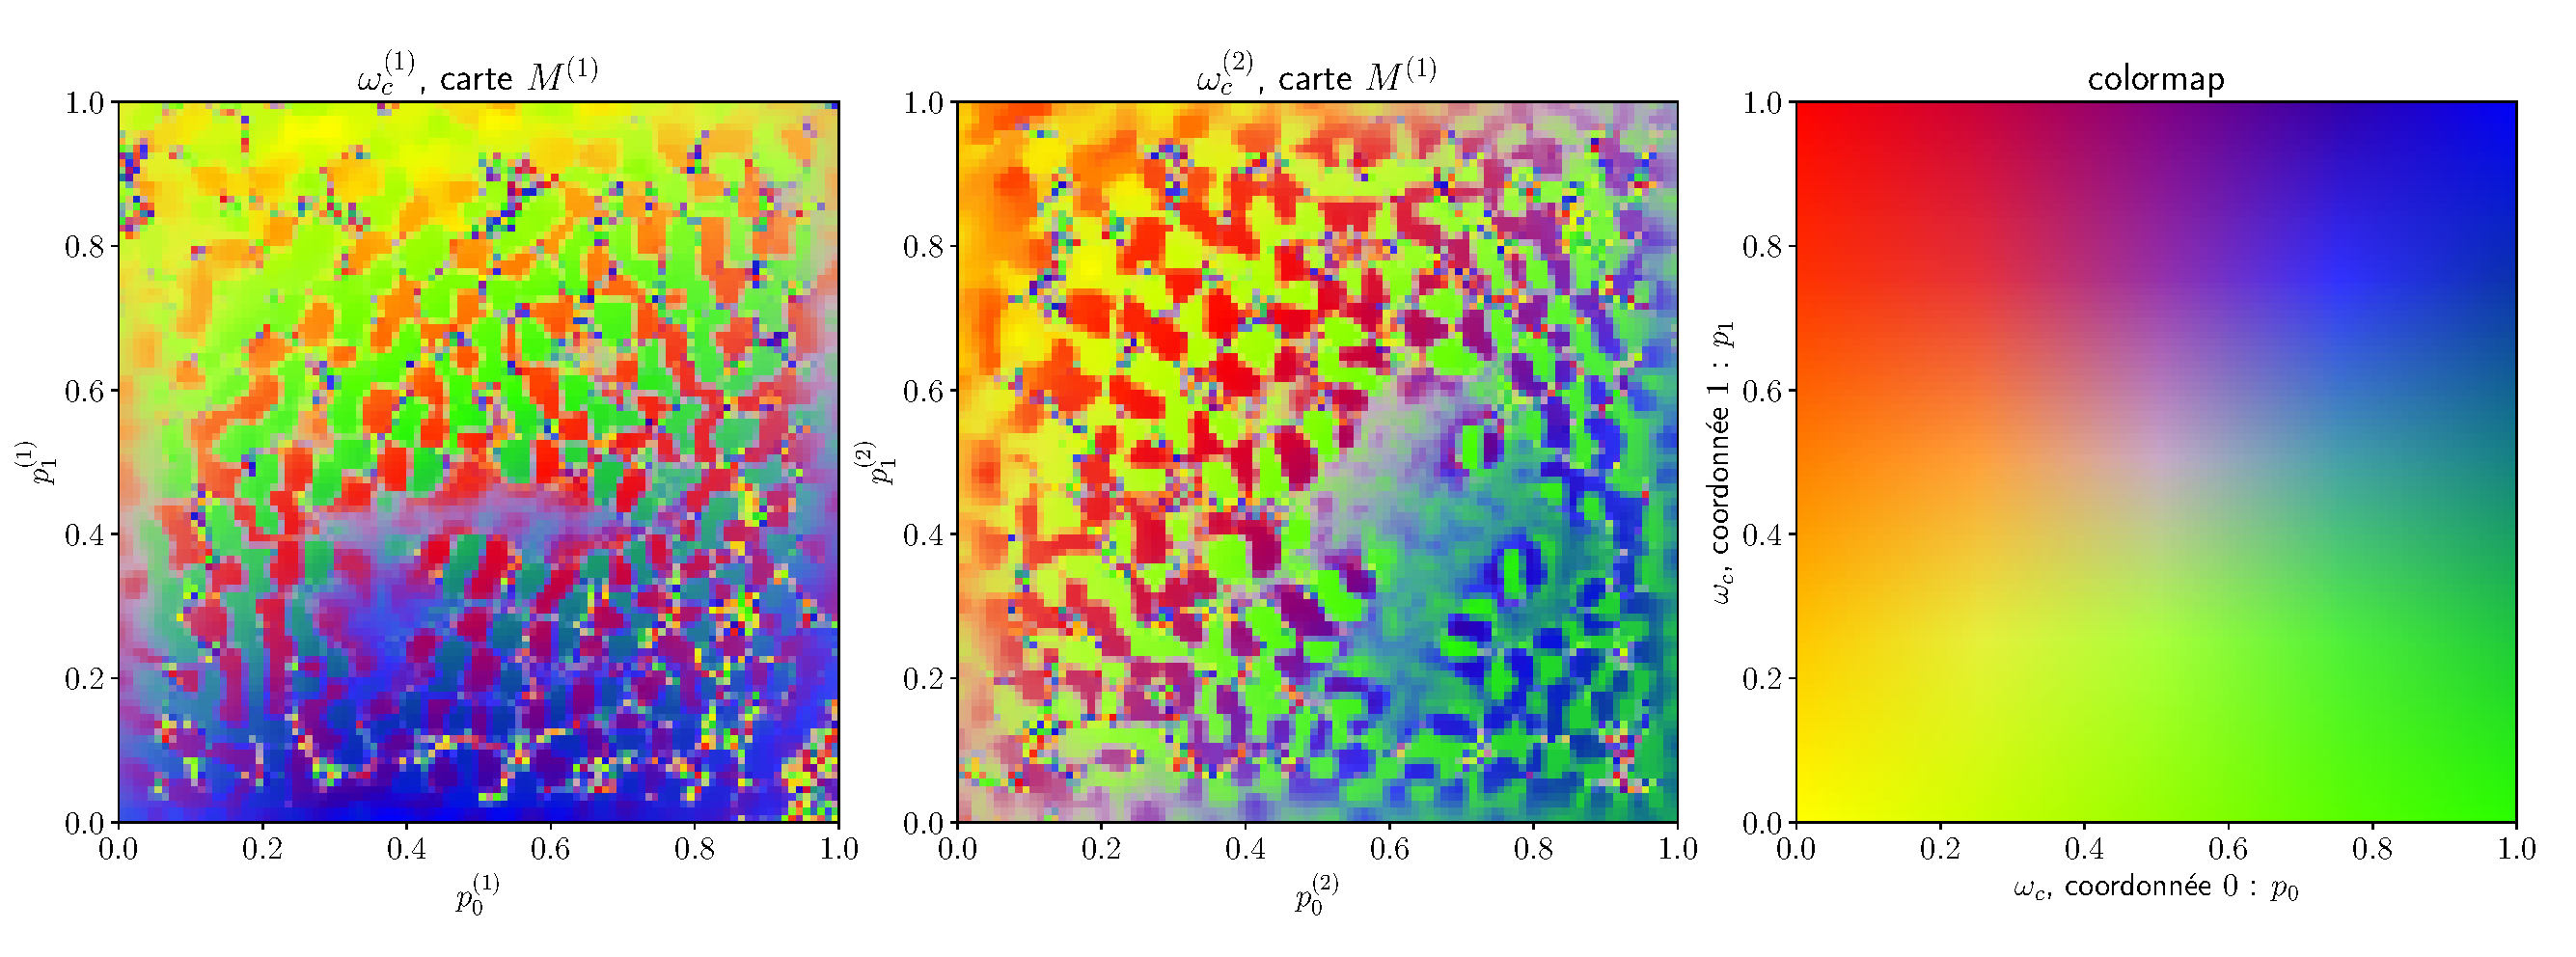
\includegraphics[width=\textwidth]{wc_rc002_afterbug_nopoints.pdf}
	\end{minipage}
	\begin{minipage}{\textwidth}
		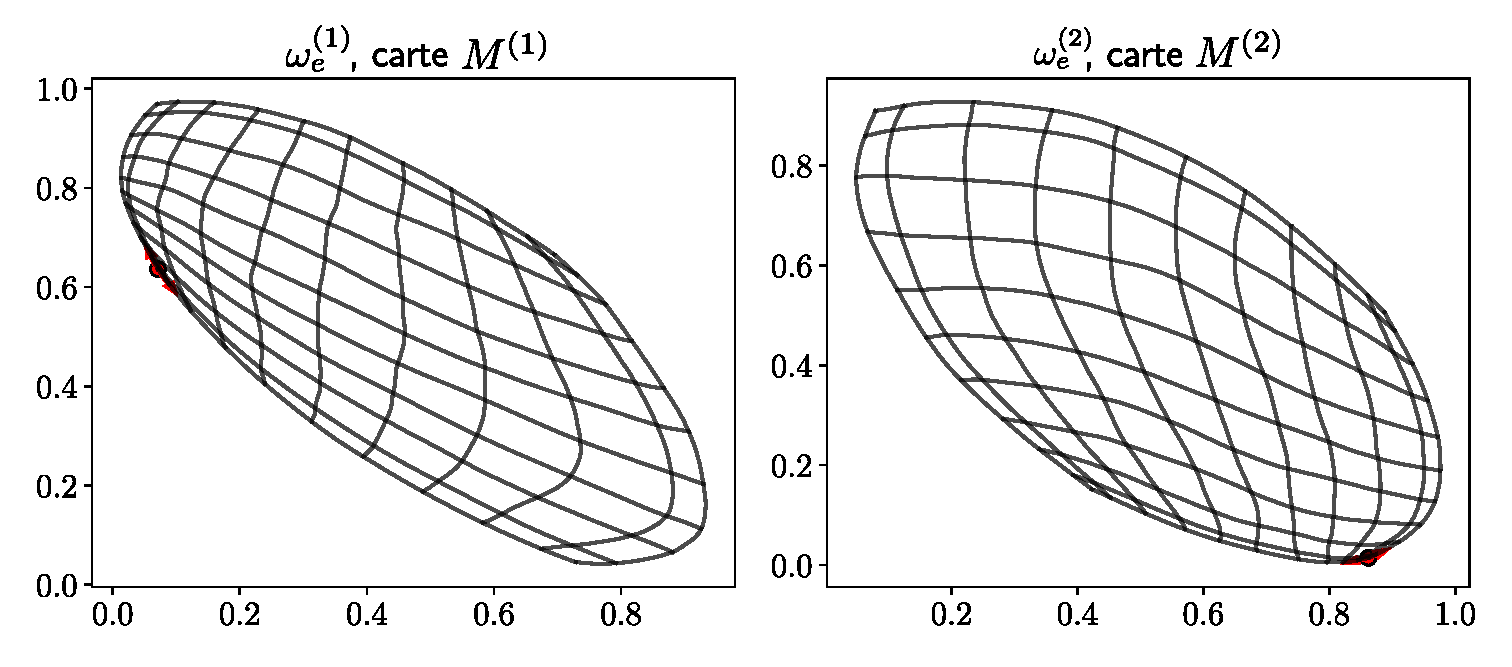
\includegraphics[width=0.7\textwidth]{we_rc002_afterbug_step10.pdf}
		\caption{Tracé des poids externes contextuels d'une architecture de cartes, organisées sur une sphère dans un espace 4D, avec $r_e =0.2$ et $r_c = 0.02$.
		En haut, les poids externes sont positionnés en fonction de leur valeur $\w_e|_x, \w_e|_y$ et reliés aux n\oe{}uds voisins. Pour une raison de lisibilité, nous avons représenté seulement une partie des connexions, les cartes étant de taille $100 \times 100$. Le coin de position $(0,0)$ de la carte est marqué par le point rouge. Cette représentation permet d'observer directement que les poids externes de chaque carte se déplient sur les entrées externes qui lui ont été présentées, dont on retrouve le tracé en figure ~\ref{fig:sphere_inputs}.
		En bas, nous traçons la valeur des poids contextuels. Nous colorons le point situé en position $p|_x, p|_y$ de chaque carte en fonction de la valeur 2D de son poids externe. Cette représentation fait apparaître une organisation en zones alternant valeurs hautes et basses sur la carte, rappelant le comportement observé en 1D.
		\label{fig:2som_s_002_wc}}
		\end{minipage}
\end{figure}

\subsection{Disposition de $U$ selon le BMU \label{par:U_bmu2D}}

Nous nous intéressons ensuite à l'apprentissage du modèle $U$ dans chacune des carte sur la disposition d'entrées en sphère afin de vérifier si chaque carte sépare les BMUs en fonction de la valeur de $U$ et non seulement de l'entrée externe.
Comme en 1D, nous pouvons tracer la valeur de $U$ selon la position du BMU dans chaque carte sur une étape de test lancée sur la configuration des poids après apprentissage.
Nous avions observé en 1D que deux zones proches codent pour des valeurs de $\inpx$ proches mais pour des $U$ différents. Dans chaque carte, $U$ est une fonction du BMU~: cette propriété marque l'apprentissage du modèle par chacune des cartes. 

La figure $\ref{fig:U_BMU}$ présente les valeurs de la variable 2D $U$, en fonction de la position du BMU $\bmu\m{1}$ et $\bmu\m{2}$ de chaque carte. La figure de droite est la carte de coloration correspondant aux valeurs 2D de $U$.
Nous y faisons figurer deux points en rouge et bleu~: ces deux entrées ont une valeur de $\inpx\m{1}$ proche mais une valeur différente de $\inpx\m{2}$ et donc de $U$.
Nous voyons sur la figure que les comportements observés en 1D se reproduisent dans cet exemple 2D~: le tracé fait figurer des zones distinctes de BMU. Une zone correspond à une seule valeur de $U$.
% La figure fait apparaître des zones blanches, sans points~: il s'agit des zones mortes, séparant les zones de BMUs. 
Les points rouge et bleu sont envoyés dans deux zones distinctes, mais contigües dans la carte $M\m{1}$. Ce comportement est donc bien équivalent à celui observé en 1D.
$U$ apparaît comme une fonction de $\bmu$ dans chaque carte. 
Nous pouvons vérifier cette propriété grâce au ratio de corrélation, dont les valeurs calculées sur CxSOM et sur des cartes simples sont indiquées au tableau \ref{tab:eta2D}. Le ratio de corrélation est calculé par le rapport entre les variances de $E(U|\bmu)$ et $E(\bmu)$. Nous prenons ici la variance au sens de moyenne des normes euclidiennes des différences à la moyenne.
Nous avions vu au chapitre~\ref{chap:indicateur} que les valeurs de ratio de corrélation doivent s'interpréter en les comparant aux valeurs prises dans une architecture de cartes indépendantes. Nous observons un ratio de corrélation de 0.99 dans chaque carte, marquant une relation fonctionnelle entre $U$ et $\bmu$. Cette valeur est plus élevée que la relation initiale entre $U$ et chaque modalité, donc une relation entre entrées est encodée par la carte.
Nous pouvons vérifier au passage la pertinence de l'utilisation du ratio de corrélation comme indicateur de l'apprentissage.
Les valeurs de ratio de corrélation sont initialement fortes~: $\eta(U;\inpx\m{2}) = 0.94$. Bien que les zones de BMUs soient clairement visibles sur la carte $M\m{2}$, en comparaison à la disposition initiale des entrées qu'on peut voir sur la figure \ref{fig:sphere_inputs}, le ratio de corrélation marque mal cette distinction. En plus grande dimension, cet indicateur est donc mal adapté. 

\begin{figure}[ht]
	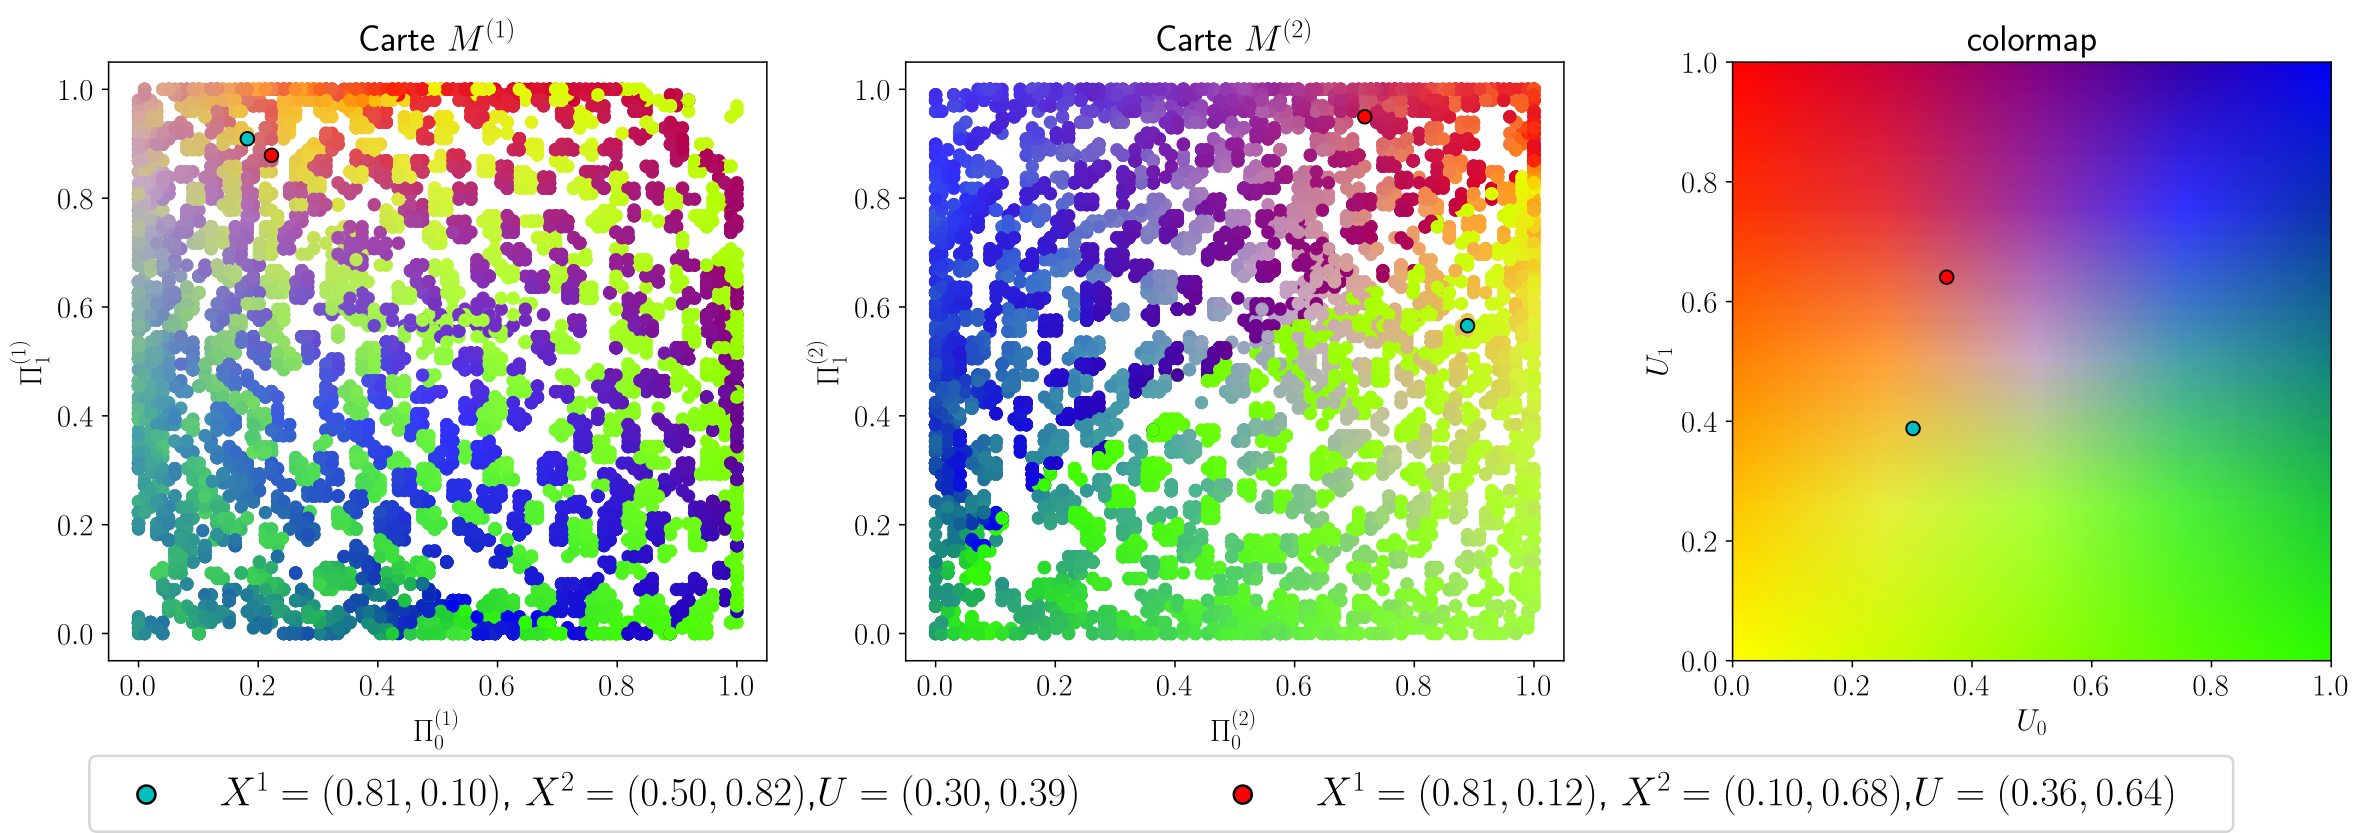
\includegraphics[width=\textwidth]{U_BMU_2SOM_2D.png}
	\caption{Disposition des valeurs de $U$, ici une variable en deux dimensions, selon les valeurs du BMU $\bmu$ dans chaque carte. Les tracés font apparaître que des zones de BMUs se spécialisent pour une valeur de $U$, comme ce qui était observé en une dimension. Les points mis en valeurs en rouge et bleu ont des valeurs très proches d'entrée $X\m{1}$, mais des valeurs différentes pour $U$ et donc $\inpx\m{2}$. Leurs BMUs sont séparés sur la carte $M\m{1}$ et envoyés dans des zones distinctes.
	\label{fig:U_BMU}}
\end{figure}


\begin{table}[hb]
	\caption{Tableau de comparaison des valeurs de $\eta$ obtenues sur la disposition d'entrées sphère. \label{tab:eta2D}}
	\centering\begin{tabular}{lcc}
						&$M\m{1}$ 					& $M\m{2}$ 						\\
		Entrées 		& $\eta(U;\inpx\m{1}) = 0.81$ & $\eta(U;\inpx\m{2}) = 0.94$  \\
		CxSOM  	 		& $\eta(U;\bmu\m{1}) = 0.98$ & $\eta(U;\bmu\m{1}) = 0.98$ 	\\
	\end{tabular}
\end{table}

\subsection{Dépendance des motifs de poids contextuels aux paramètres des cartes \label{par:params2D}}

La formation de zones de poids contextuels dépend des paramètres de la carte, en particulier du rapport entre les rayons de voisinage.
Nous comparons dans cette section la forme des motifs de poids contextuels pour une même taille de $r_e$ mais des rayons de poids contextuels $r_c$ différents.
Nous nous demanderons également si les poids contextuels et externes convergent dans ces configuration de paramètres.
Les Figures~\ref{fig:rc_002}, \ref{fig:rc_003} et \ref{fig:rc_005} présentent l'évolution des poids contextuels au cours de l'apprentissage pour une même distribution de données d'entrées sur une sphère 3D, $r_e = 0.2$ et $r_c = 0.02, 0.03$ et $0.05$
Nous remarquons que l'expérience avec $r_c = 0.02$ conduit à une configuration stable des poids contextuels, \ref{fig:rc_002}. 
La convergence est également observée dans l'expérience avec $r_c = 0.03$ en figure \ref{fig:rc_003}. Au contraire, nous n'observons pas de convergence pour $r_c =0.05$~: à l'issue des 500 000 itérations, nous continuons à observer des changements dans la structure des poids contextuels. 
Dans les deux premiers cas, les poids contextuels forment des motifs en zones. La taille de ces motifs dépend de la valeur de $r_c$. Ces motifs ne sont pas observés dans le cas $r_c = 0.05$. 
Sur cette figure, nous représentons également la valeur des poids contextuels de chaque carte par les grille blanche et noire sur la carte de coloration. Les points  correspondent aux valeurs prises par les poids $w_c$ dans chaque carte, reliés selon leur voisinage.
Nous voyons ici que les poids contextuels ne se sont pas dépliés sur toutes les positions $[0,1]^2$, alors que c'était le cas pour les deux configurations de paramètres précédentes.
En 1D, nous avions noté que les zones ne se forment qu'en dessous d'une certaine valeur de $\frac{r_e}{r_c}$.
C'est également ce qui est observé ici, les zones se formant en dessous d'une valeur se situant entre $r_e = 10 r_c$ et $r_e = 6 r_c$.
% En Figure~\ref{fig:conv_poids}, nous avons tenté de représenter l'évolution des poids au cours de l'apprentissage, en traçant, tous les 5000 itérations, la moyenne des différences entre les poids des cartes au temps courant $t$ et à la dernière configuration observée ($t - 5000$). Ce tracé ne constitue pas une preuve expérimentale de convergence, mais nous donne une idée de l'évolution des poids observée à l'\oe{}il. Pour $r_c = 0.02$, nous relevons une différence moyenne entre les poids au temps $t$ de 0.01 à l'itération 500000.
% Plusieurs travaux dans la littérature proposent des outils et des critères pour étudier la convergence et l'organisation de cartes de Kohonen \cite{Polani2001MeasuresFT, Breard2017EvaluatingSM, Tatoian2018SelfOrganizingMC}, qu'il serait intéressant d'utiliser également dans les architectures CxSOM.
Nous pouvons conclure de ces observations préliminaires en deux dimensions que la formation de zones est un mécanisme qu'on retrouve dans des cartes 1D comme des cartes 2D. Ces zones dépendent comme en 1D du rapport entre rayons de voisinage externe et contextuels.

L'aspect 2D apporte beaucoup moins de contraintes sur la forme des zones que sur des cartes en une dimension, rendant possible la formation différents motifs sur les poids contextuels. 
Contrairement au cas en une dimension dans lequel la convergence des poids était assurée, la convergence des poids contextuels dans une carte 2D n'est pas assurée en fonction des paramètres de la carte. Cette étude paramétrique en deux dimensions apparaît comme une suite nécessaire de l'étude des cartes.
Nous avons analysé la forme des poids sur un seul type de distribution, une sphère dans un espace 4D, pour différents rayons de voisinage de la carte. Nous observons que les motifs formés par les poids contextuels sont similaires dans les deux cas $r_c = 0.02$ et $r_c = 0.03$ et ne dépendent pas des conditions initiales des expériences~: les poids des cartes sont initialisés aléatoirement de façon différente dans chaque expérience et les entrées sont tirées sur une même distribution de façon aléatoire.
Nous pouvons donc supposer que comme en 1D, le type de relation entre entrées influence l'organisation des motifs des poids contextuels. L'observation de comportements d'une carte 2D en fonction du type d'entrées présentées peut également constituer une suite pertinente de ces résultats préliminaires.

\begin{figure}[p]
	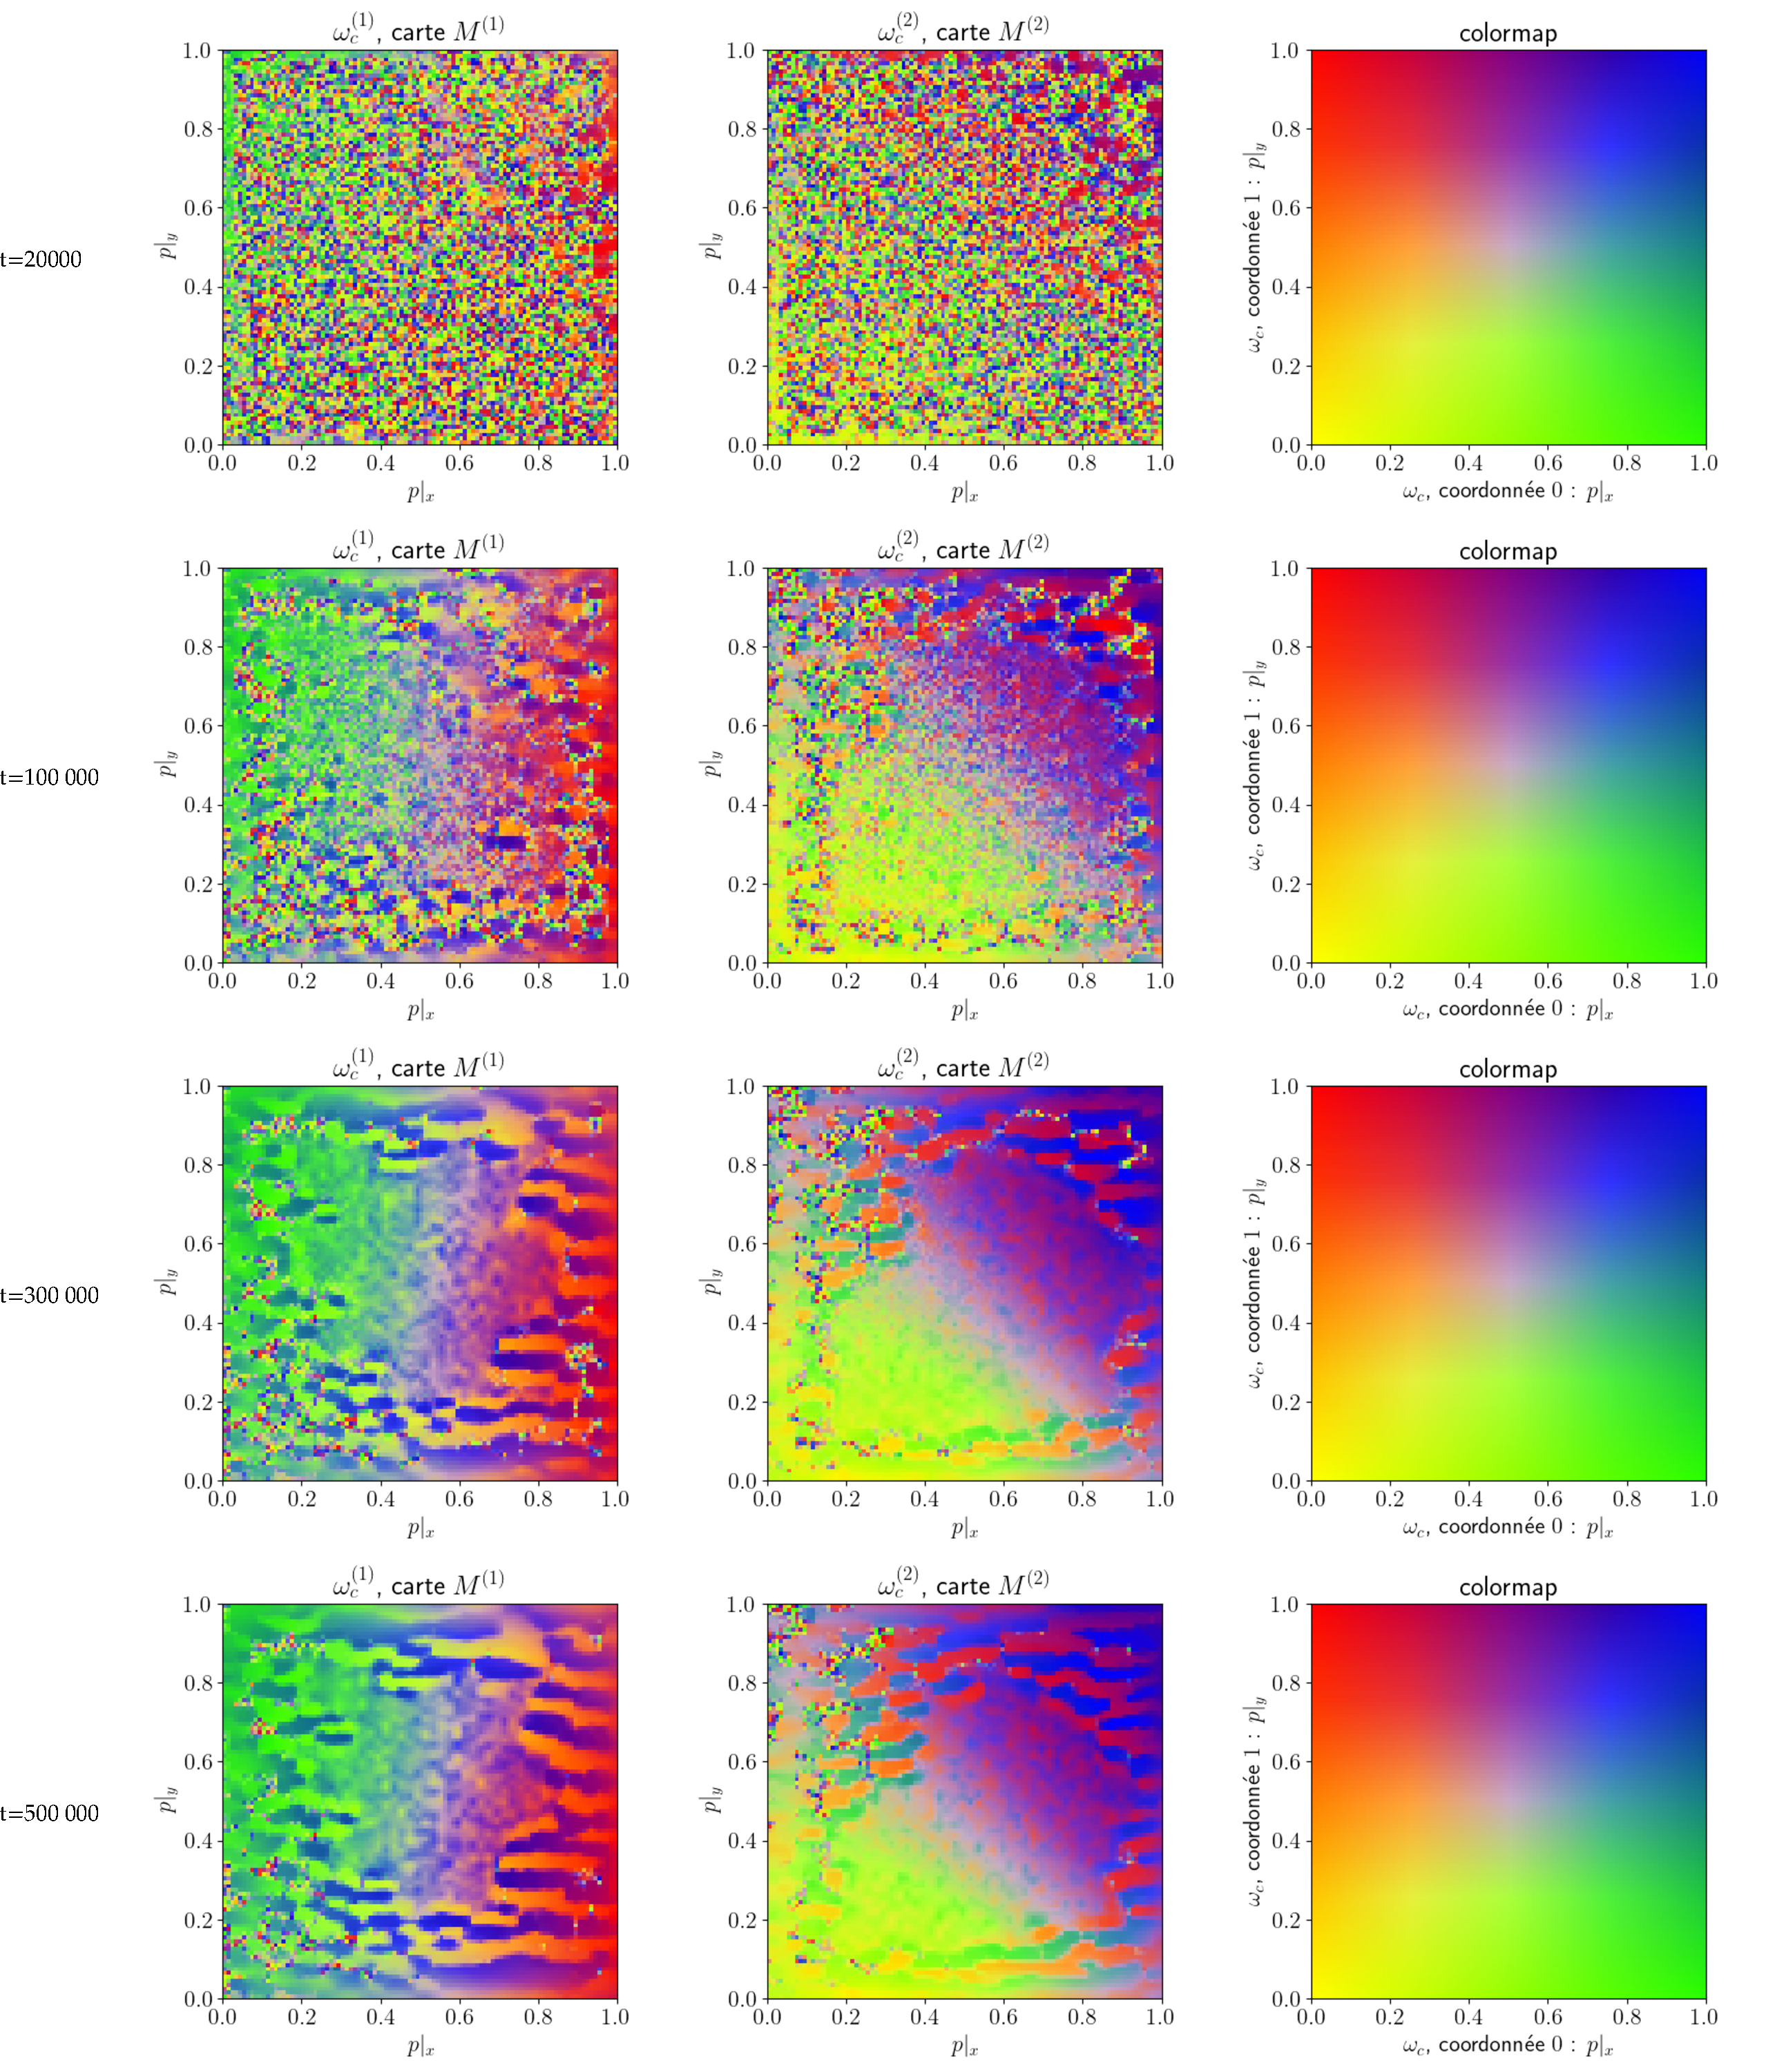
\includegraphics[width=\textwidth]{2SOM_sphere_rc002_evol.pdf}
	\caption{\'Evolution des poids contextuels d'une architecture de deux cartes pour $r_c =0.02$. Les poids contextuels évoluent vers une position stable, formant des motifs alternant valeurs hautes et basses des poids contextuels. La zone centrale est constituée d'une alternance  \label{fig:rc_002}}
\end{figure}

\begin{figure}[p]
	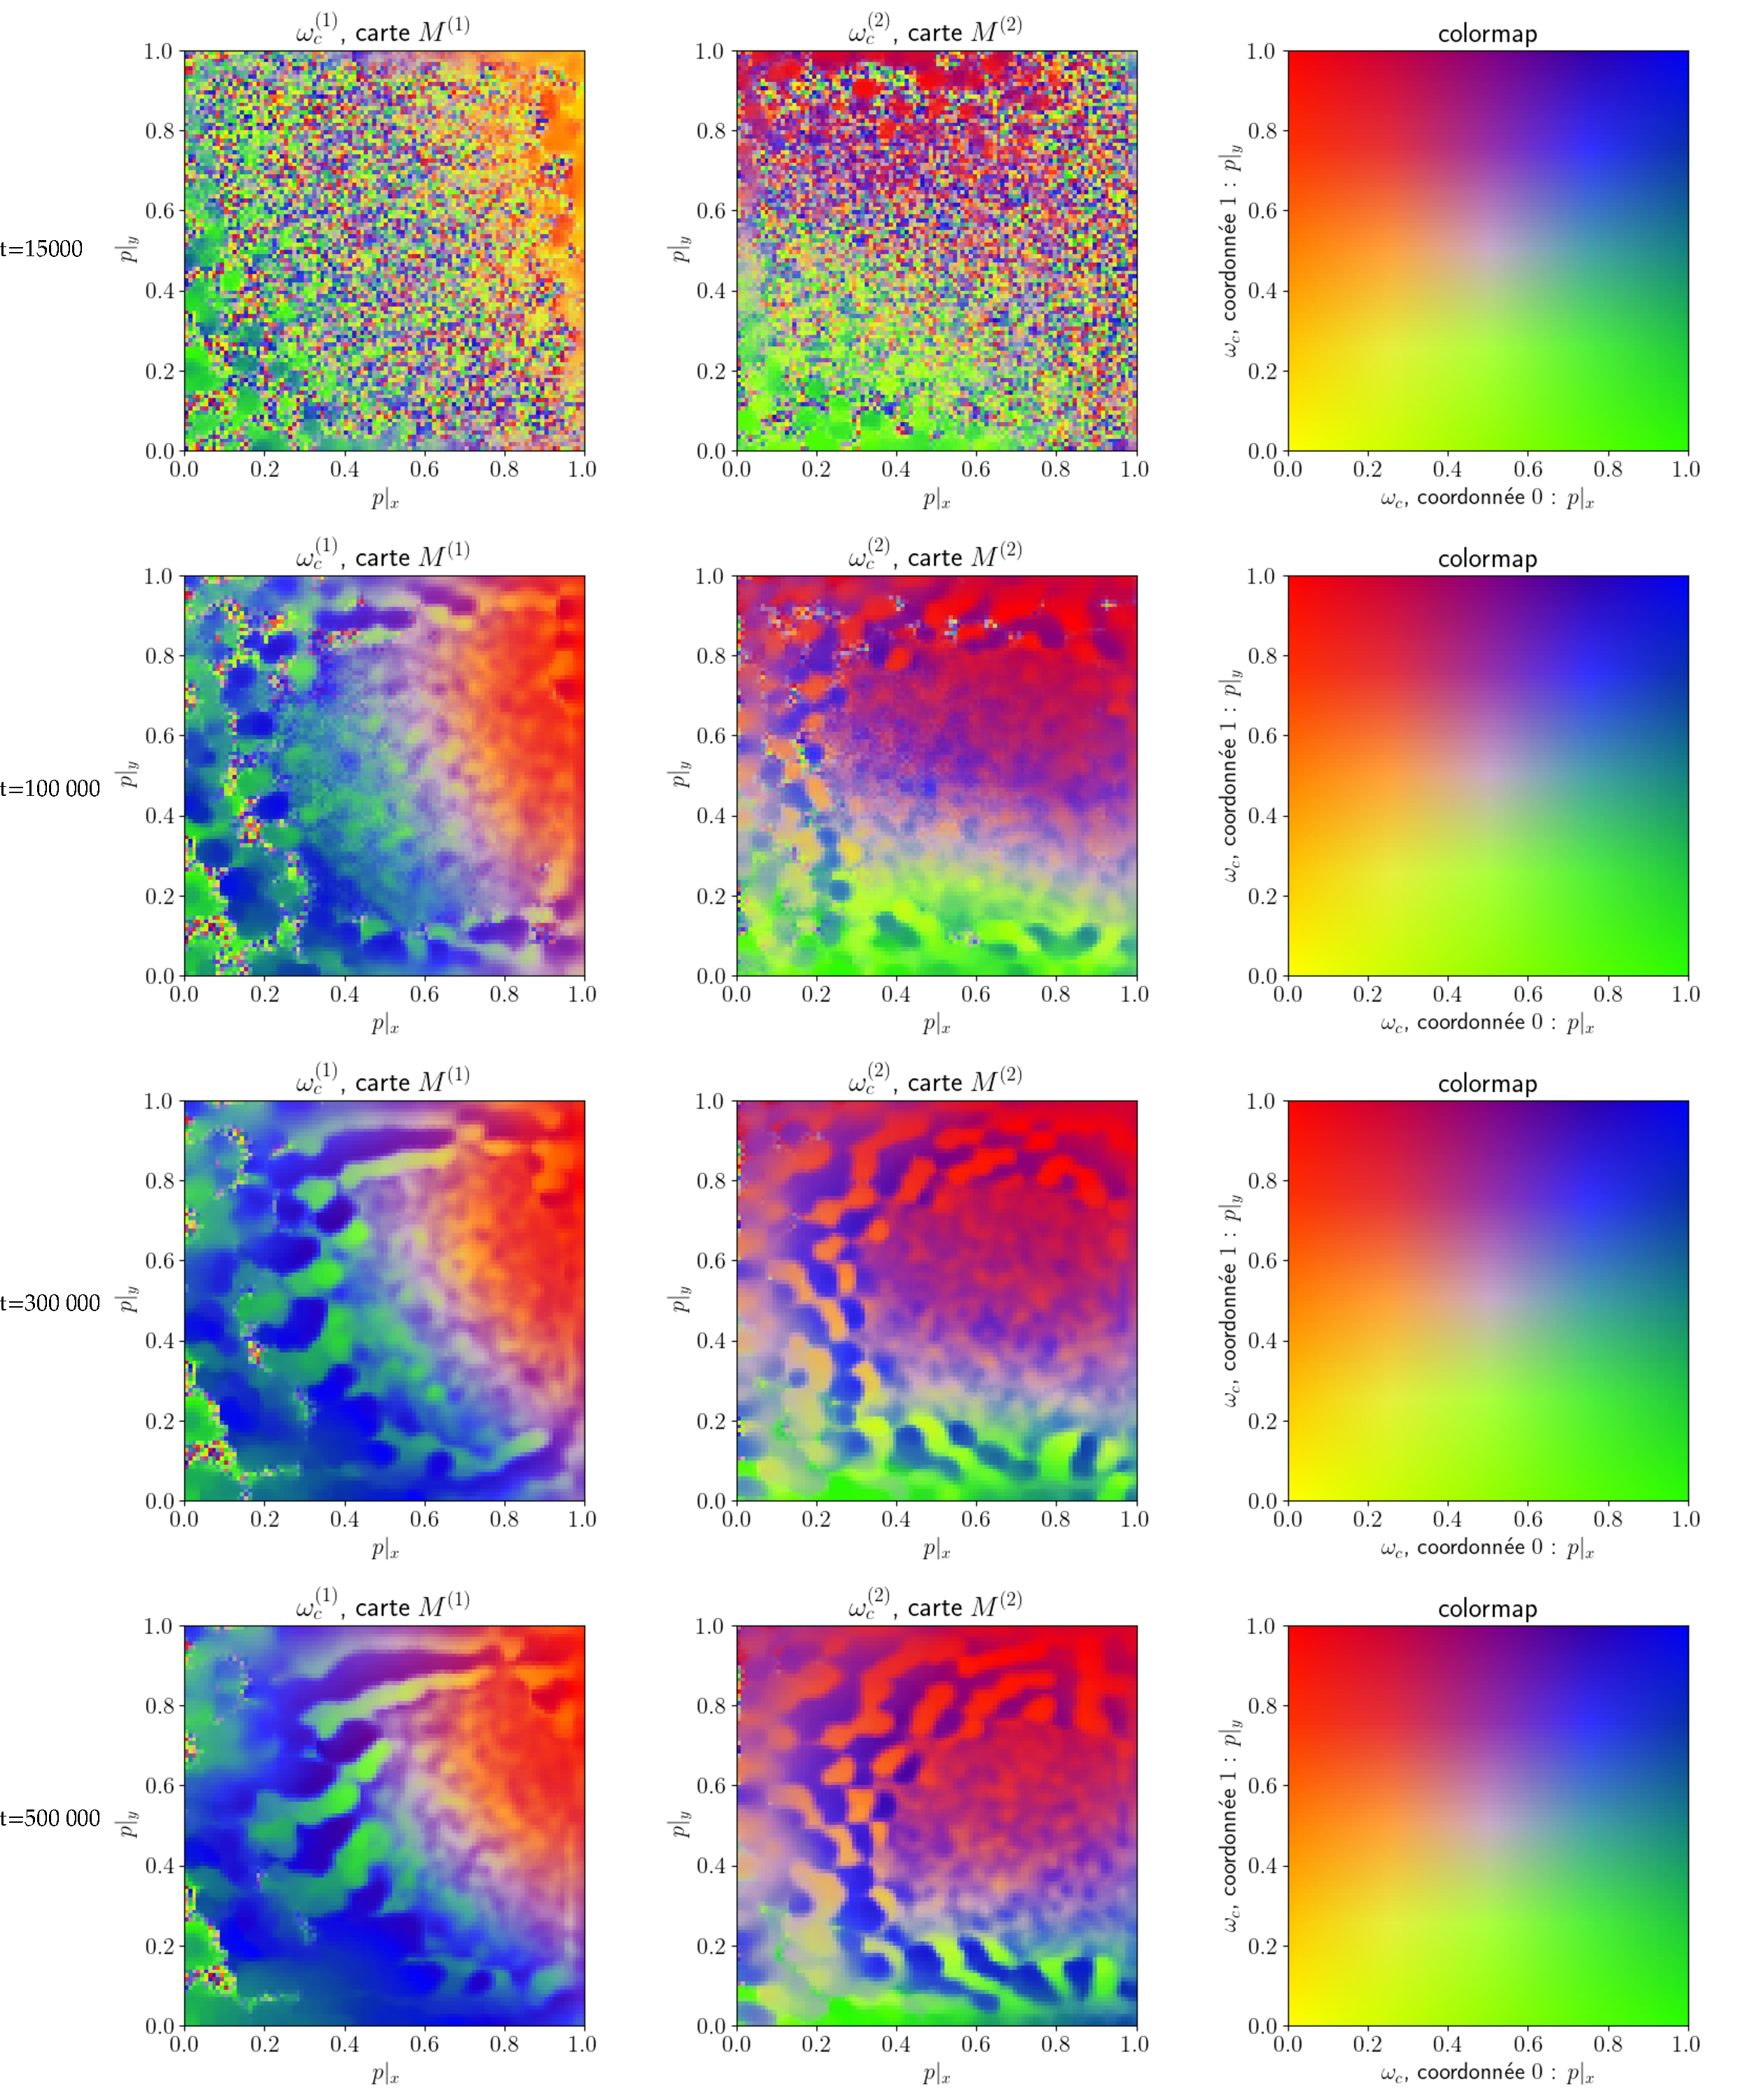
\includegraphics[width=\textwidth]{2SOM_sphere_rc003_evol.pdf}
	\caption{\'Evolution des poids contextuels d'une architecture de deux cartes pour $r_c =0.03$. Les motifs observés sont similaires à ceux observés pour $r_c = 0.02$. La taille des motifs est plus large. \label{fig:rc_003}}
\end{figure}

\begin{figure}[p]
	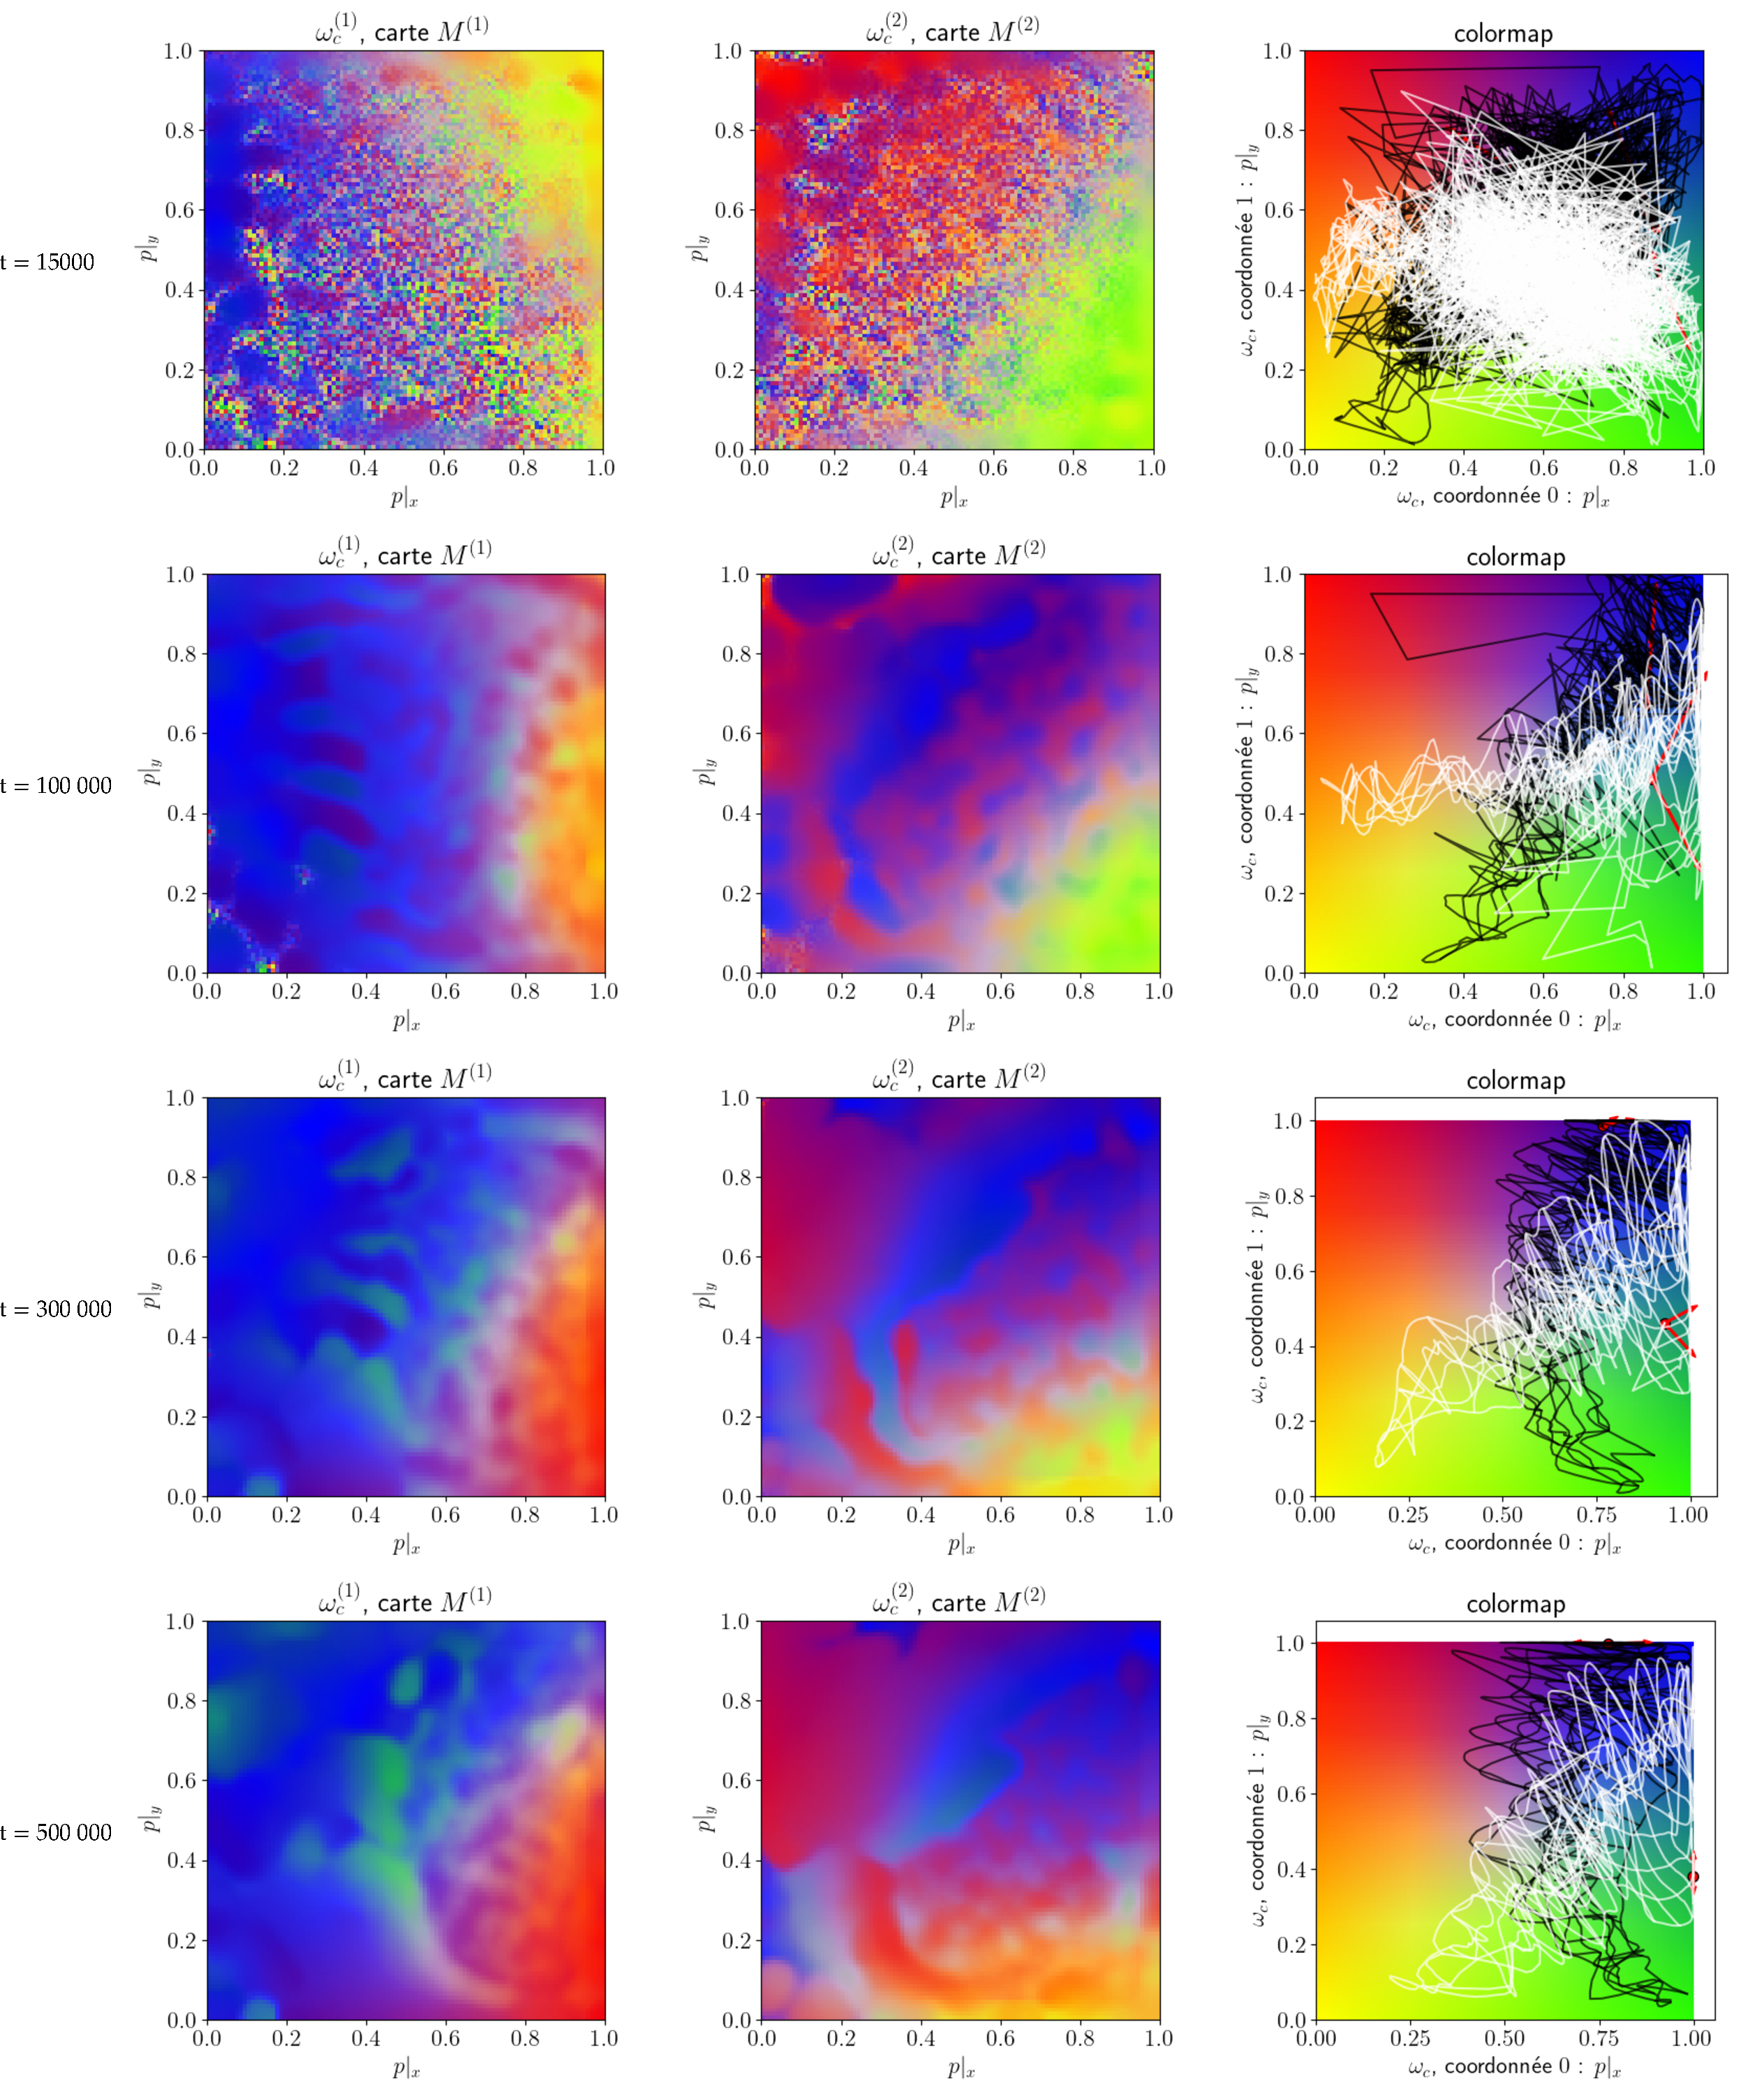
\includegraphics[width=\textwidth]{2SOM_sphere_rc005_evol}
	\caption{\'Evolution des poids contextuels d'une architecture de deux cartes pour $r_c =0.05$. 
	Nous remarquons que les poids contextuels se déplient sans occuper tout l'espace des positions, ce qui est marqué par la disposition de la grille. Ce dépliement est mis en valeur sous forme de disposition en grille dans l'espace des positions sur la figure de droite : $\w_c\m{1}$ en noir et $\w_c\m{2}$ en blanc. Par ailleurs, nous n'observons pas de convergence claire des poids contextuels. Les grilles noires et blanches continuent d'évoluer après 700 000 itérations.
	Ce comportement rappelle ce qui est observé en 1D. Pour un rayon de voisinage $r_c$ trop grand, les poids contextuels ne forment pas de zones. C'est ce qui est observé dans ce cas en 2D.
	\label{fig:rc_005}}
\end{figure}


% \begin{figure}
% 	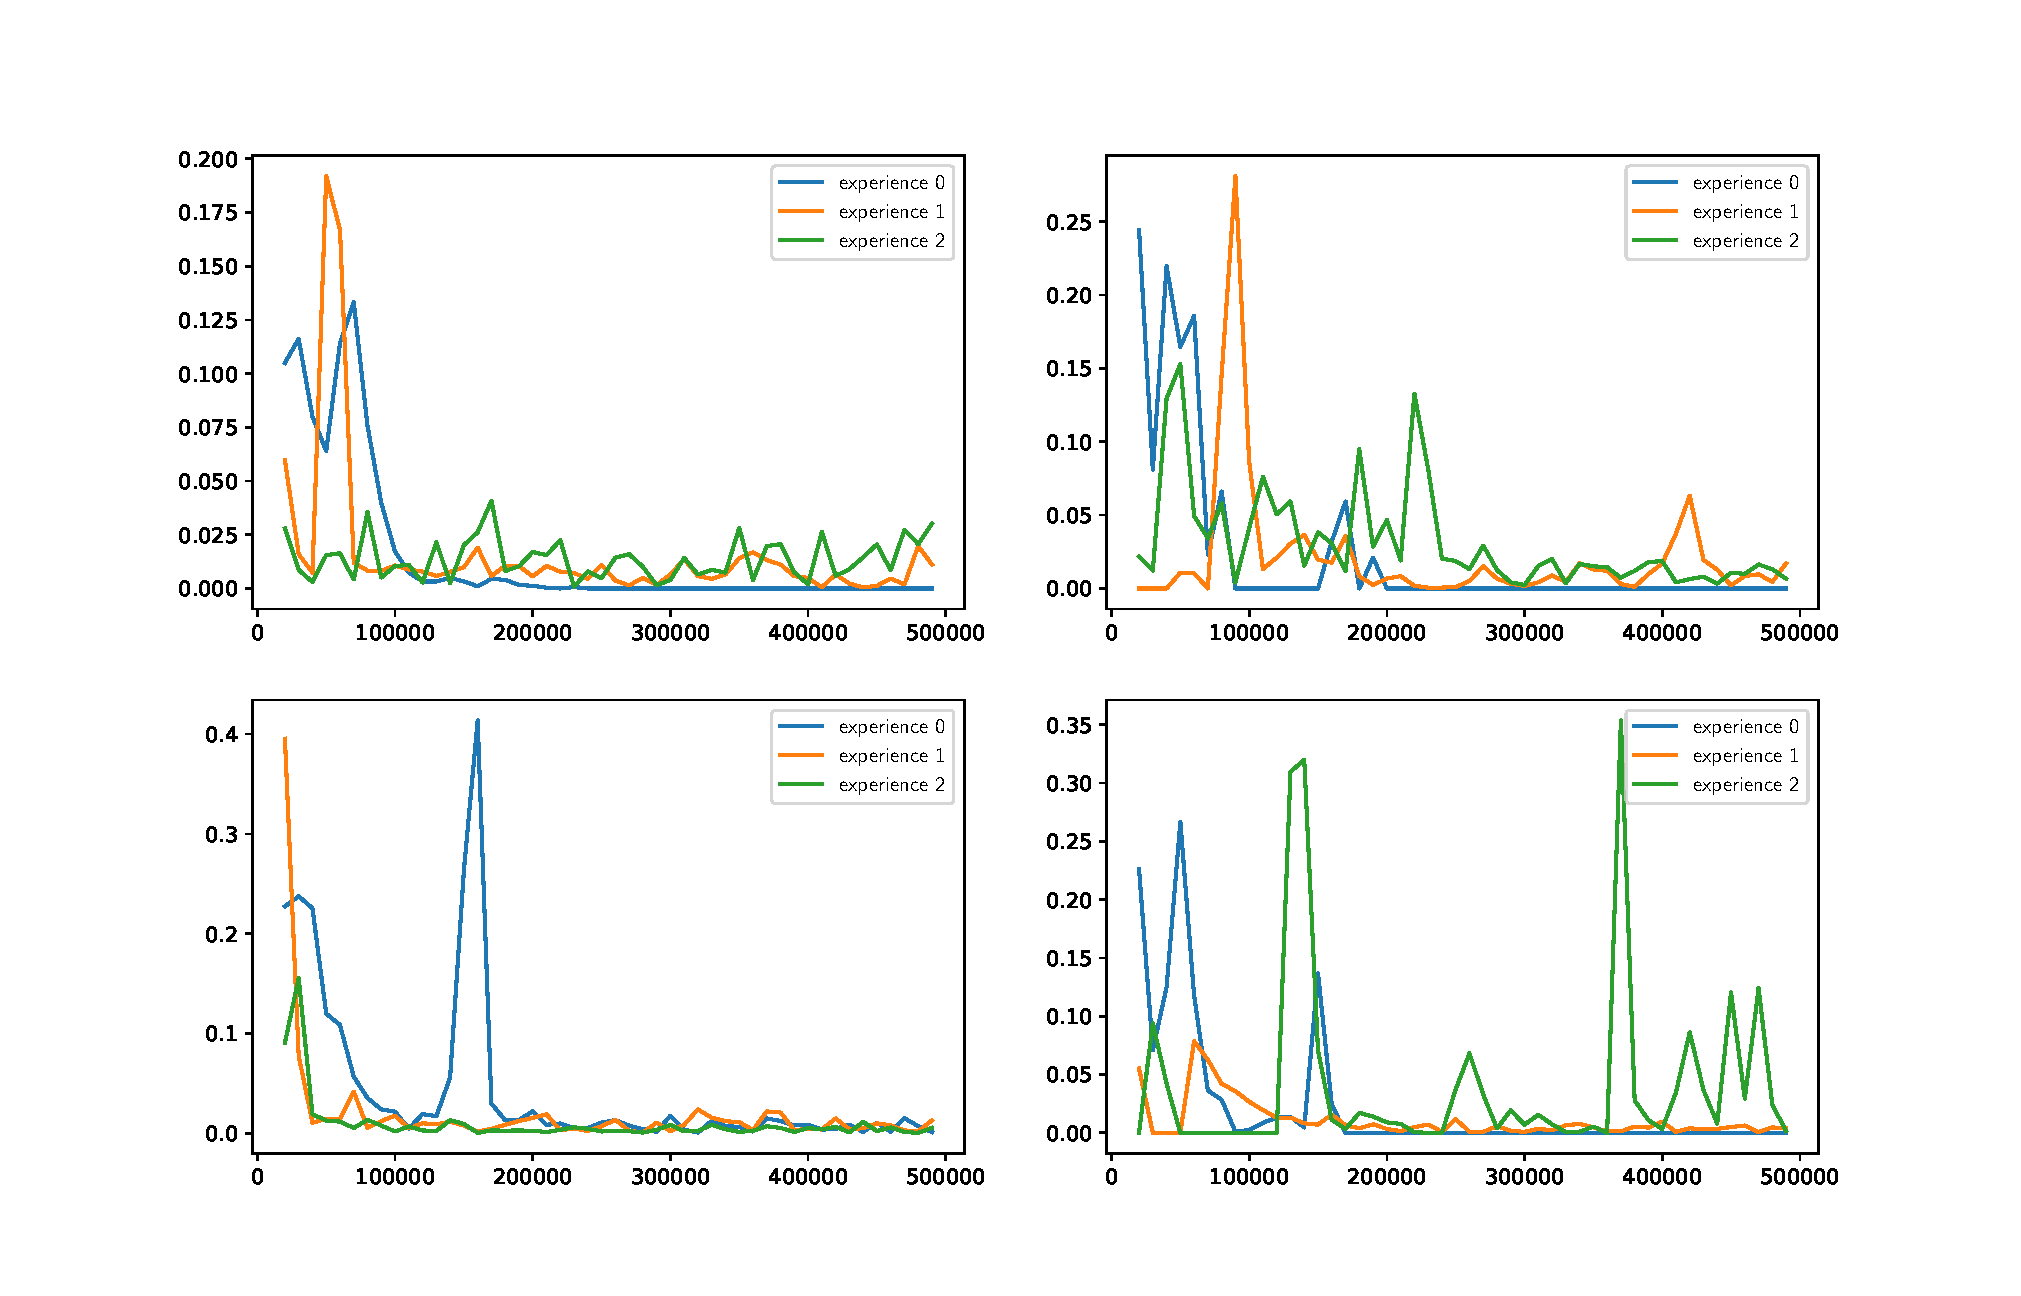
\includegraphics[width=\textwidth]{evol_convergence_poids.pdf}
% 	\caption{\'Evolution de la différence moyenne entre les poids externes et contextuels au cours de l'apprentissage d'une architecture de 2 cartes sur une sphère 3D en 4 dimensions. Le calcul de différences est réalisé toutes les 10 000 itérations. Nous avons tracé les courbes pour 4 expériences avec $r_e = 0.2$ et $r_c = 0.02$ ainsi que pour les expériences avec $r_e = 0.2$ et $r_c = 0.05$,$r_e = 0.2$ et $r_c = 0.03$. Nous remarquons que cette différence évolue vers une valeur faible, qu'on attend nulle pour une carte stabilisée. Ici les poids tendent vers une valeur faible qui semble stable. Notons que cela ne montre pas forcément la convergence~: les poids peuvent se déplacer faiblement dans une même direction. Le tracé nous assure simplement que l'évolution des poids est lente en fin d'apprentissage. \label{fig:conv_poids}}
% \end{figure}

\subsection{Convergence de la relaxation \label{par:conv2D}}

Nous nous intéressons ensuite à la convergence de la relaxation sur l'expérience en deux dimensions. 
Nous traçons en figure \label{fig:relax2D} l'évolution du taux de convergence des tests au cours de l'apprentissage pour des structures de deux cartes en deux dimensions, par le processus décrit au chapitre \ref{chap:relax}. Lors de plusieurs phases de test lancées à des itérations $t$ au cours de l'apprentissage, nous comptons le nombre de pas nécessaires à la convergence de la recherche de BMU par relaxation et traçons sur la figure la moyenne de ce nombre de pas de relaxation, à différents temps d'apprentissage $t$.
Nous traçons également le taux d'échantillons d'une phase de test menant à une convergence de la relaxation. On considère que la relaxation n'a pas convergé si le nombre de pas atteint le seuil maximal de 1000 pas fixé par notre étude. Le nombre de pas de relaxation moyen étant observé de 20 pas, ce seuil est pertinent pour considérer que la relaxation n'a pas convergé.
Nous traçons ces évolutions pour les différentes configurations de paramètres de cartes~: nous avons réalisé trois expériences de mêmes paramètres $r_e=0.2$ et $r_c = 0.02$, une expérience avec $r_c = 0.03$ et une avec $r_c = 0.05$ Dans cette dernière expérience, les poids n'ont pas formé de zones distinctes (voir figure \ref{fig:rc_005_evol}.
Nous voyons que la relaxation converge bien dans entre 95 et 98 \% des cas tout au long de l'apprentissage. Comme dans les cartes 1D, la relaxation converge peu lorsque les poids ne sont pas organisés et le taux de convergence augmente au cours de l'organisation des cartes.
Les valeurs trouvées pour $r_c = 0.05$ sont similaires au cas $r_c = 0.02$, dans lequel les poids ont bien convergé. La relaxation dans des cartes en deux dimensions n'est donc pas liée à la formation de zones stables~: la relaxation trouve un point fixe dans un cas général de cartes en 2D.
Cette observation est prometteuse pour la construction d'architectures de cartes 2D.

\begin{figure}
	\centering
	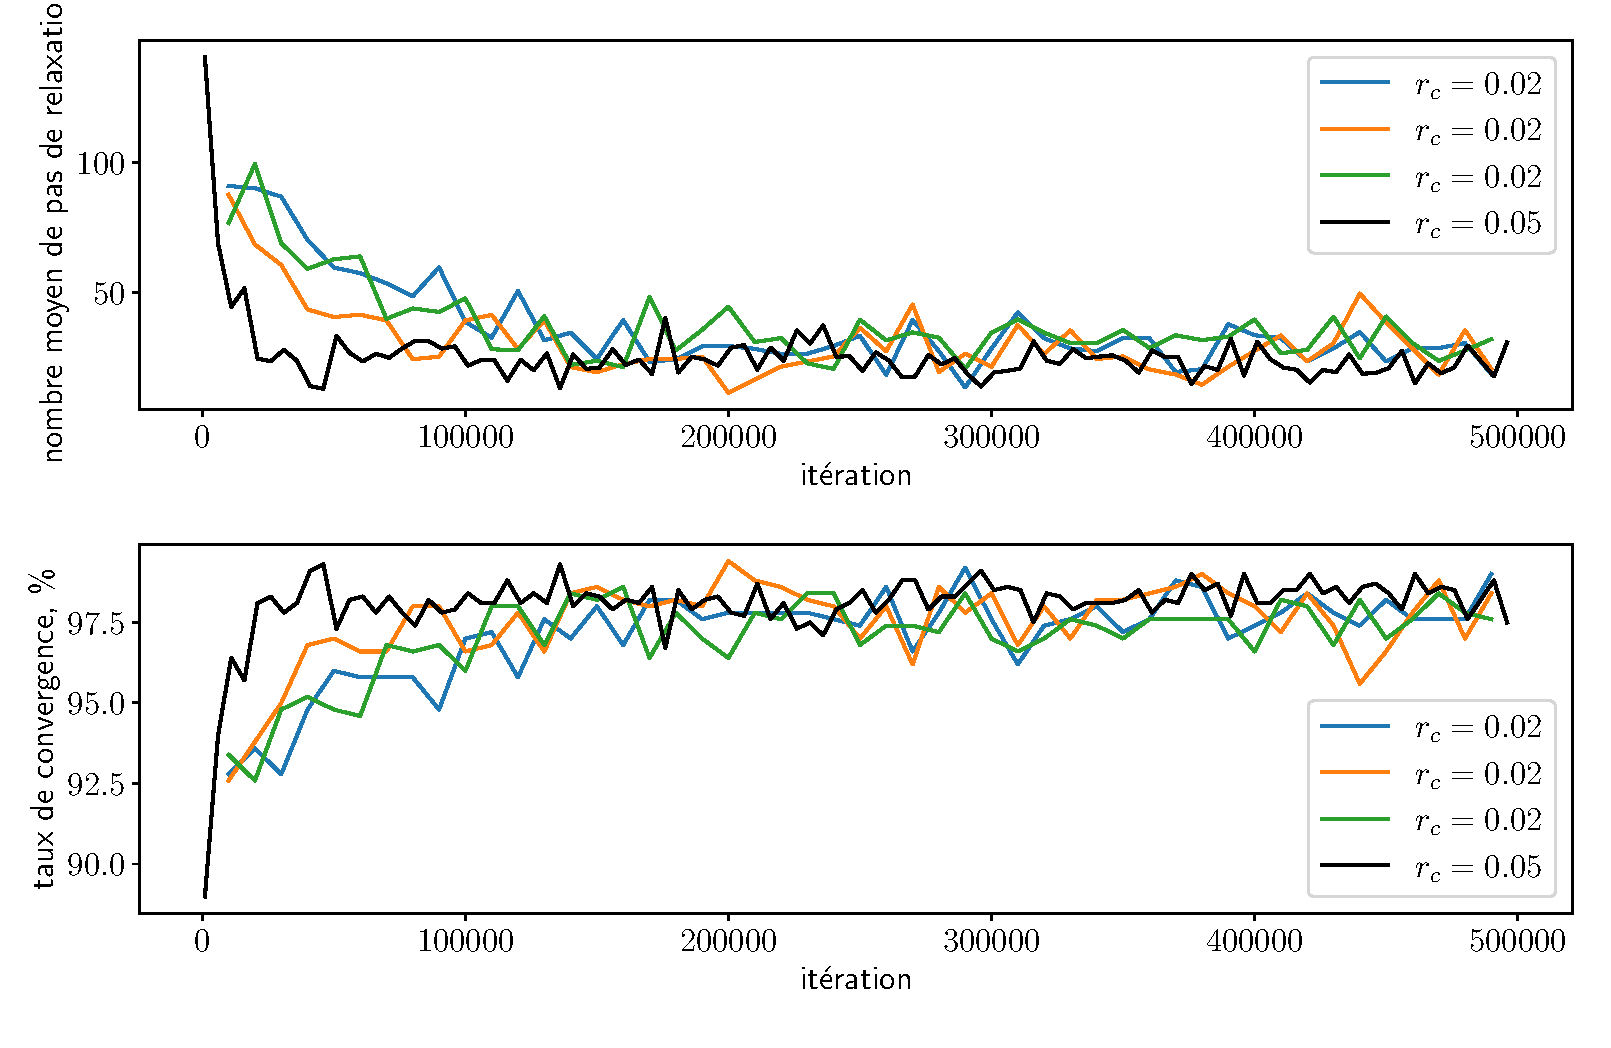
\includegraphics[width=0.8\textwidth]{conv_relax_2maps.pdf}
	\vspace{-0.5cm}
	\caption{\'Evolution de la convergence de la relaxation au cours de l'apprentissage. Nous avons réalisé les tracés sur trois expériences générées pour $r_c = 0.02$, sur des entrées aléatoires tirées sur la même distribution, une sphère plongée en 4D. Pour comparaison, nous traçons également l'évolution pour la configuration dans laquelle $r_c = 0.05$, dans laquelle les poids contextuels n'ont pas formé de zones. La relaxation converge en fin d'apprentissage~: le BMU a donc un sens dans les cartes en deux dimensions. \label{fig:relax2D}}
\end{figure}

\subsection{Organisation de cartes sur des entrées indépendantes \label{par:cub2D}}

Nous nous intéressons enfin à l'organisation d'une architecture de deux cartes prenant des entrées $\inpx\m{1}, \inpx\m{2} \in [0,1]^2 \times 0,1]^2$ indépendantes.
En 1D, nous avions observé deux échelles d'indices dans le choix des BMUs, découpant chaque carte selon la valeur de l'entrée externe. Dans chaque intervalle de ce découpage, les poids contextuels permettent de différencier le BMU selon la valeur de l'autre entrée, formant une sous -arte de toutes les valeurs de $[0,1]$ sur chaque intervalle de la carte.
Nous cherchons à observer si ces zones de BMUs sont encore présentes et si chaque zone permet de cartographier tout l'intervalle $[0,1]^2$.
Les rayons de voisinage sont pris à $r_e = 0.2, r_c = 0.02$, comme nous avons vu dans les expériences précédentes que cette configuration permet la formation de zones.

Les valeurs des poids externes et contextuels sont tracés en figure \ref{fig:2som_cub_wc}.
Les poids externes sont bien dépliés sur l'ensemble des entrées, ce qui est similaire au cas en une dimension.
Les poids contextuels restent par contre centrés autour de $0.5$, mis en évidence par les tracés en blanc et noir sur la carte de coloration à droite de la figure.
Pourtant, nous avons observé que toutes les positions d'une carte sont bien BMU lors des phases de tests. 
Les poids contextuels auraient dû, pour bien cartographier les positions sur l'autre carte, s'étendre sur tout le carré dans chaque zone.
Ce comportement de moyennage est à rapprocher du comportement limite observé sur une architecture de 10 cartes en une dimension~: nous avons vu que des architectures de 10 cartes apprenant sur 10 entrées 1D indépendantes voient également leurs poids contextuels se moyenner autour de $0.5$ dans chaque carte.
Nous pouvons proposer une interprétation de ce comportement~: lorsque les entrées présentent une  dépendance, un nombre fini ou un intervalle réduit de valeurs de $\inpx\m{2}$ seront présentées à l'architecture pour une même valeur de $\inpx\m{1}$. Cela correspond à un nombre réduit de valeurs de $\bmu\m{2}$ donc un nombre réduit d'entrées contextuelles différentes pour $M\m{1}$. 
Les poids contextuels situés autour de la position codant pour $\inpx\m{1}$ s'organisent alors comme une carte des valeurs des entrées contextuelles présentées lorsque $\inpx\m{1}$ est proche de la valeur en question. En une dimension, cette sous carte avait possibilité de s'étendre sur tout l'intervalle de valeurs de $\inpx\m{2}$, formant donc des zones distinctes. En ajoutant des entrées contextuelles, les poids tendaient vers une valeur moyenne des positions, donc 0.5.
En deux dimensions, pour une même valeur de $\inpx\m{1}$, toutes les valeurs possibles de $\inpx\m{2}$ dans le carré $[0,1]^2$ sont présentées. Les poids contextuels n'ont pas la liberté de s'étendre sur toutes ces valeurs et prennent donc une valeur moyenne.

Ce comportement peut apparaître comme une limite de CxSOM, marquant le fait que les poids contextuels manquent de liberté pour s'organiser.
Au contraire, nous pouvons aussi envisager ce comportement comme une capacité de détection de dépendance entre entrées, qui est encore plus marquée sur les cartes 2D que sur les cartes 1D. 

\begin{figure}[H]
	\centering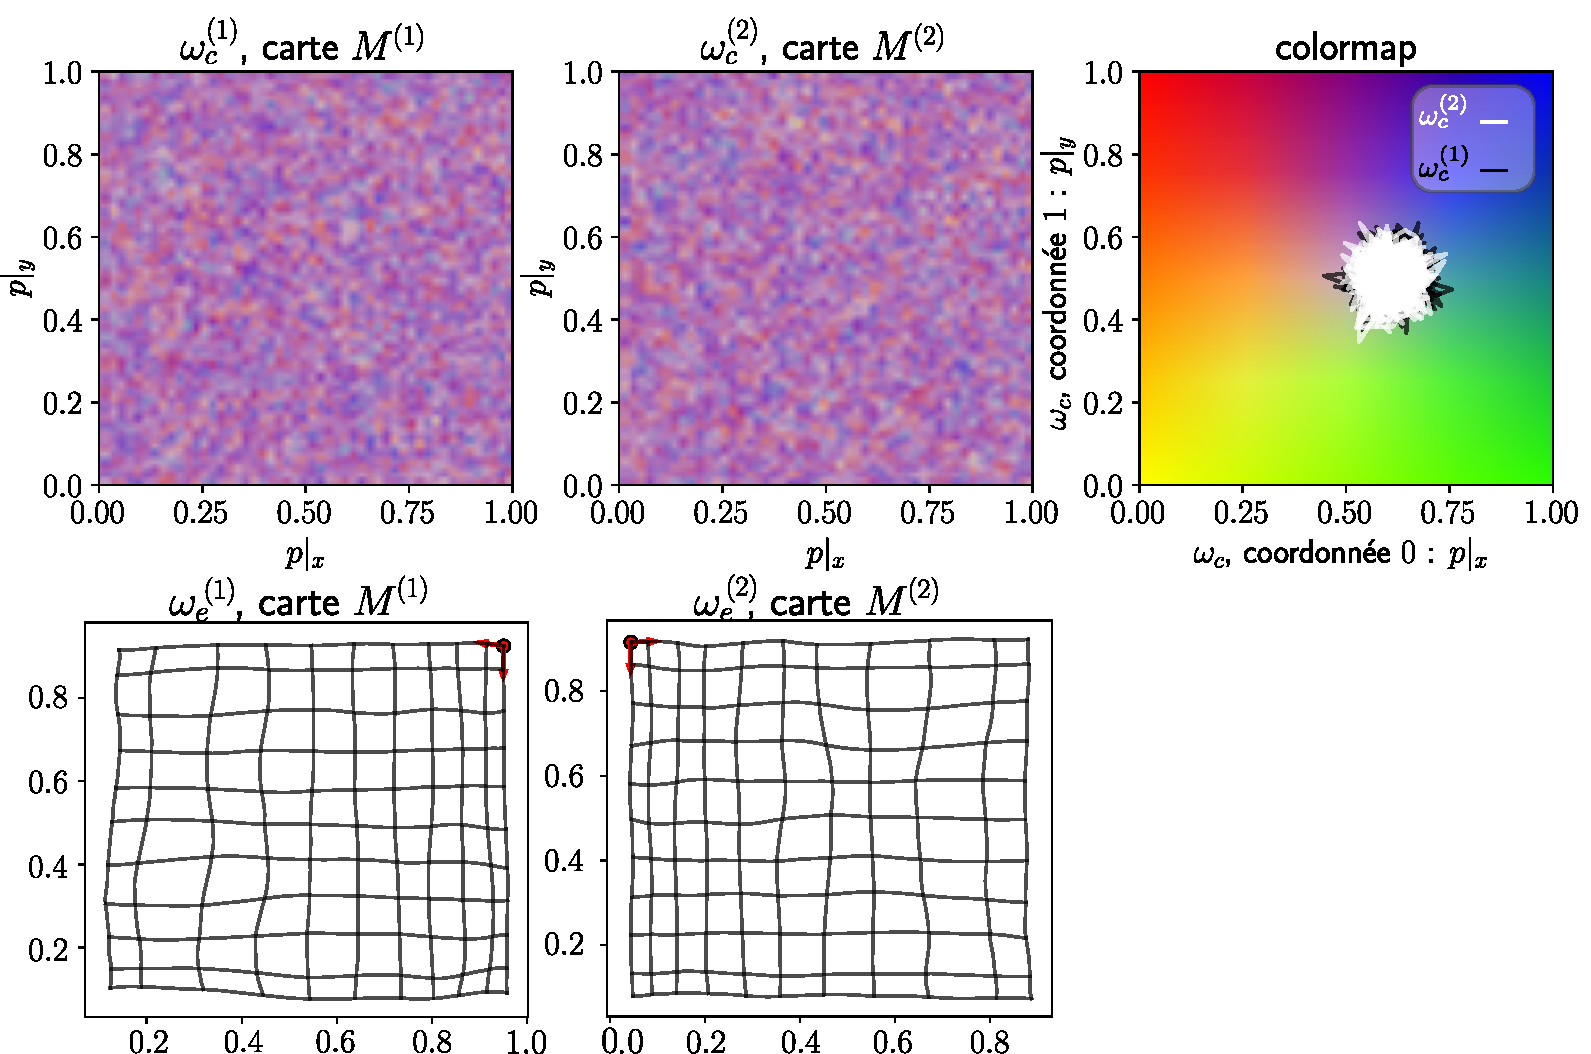
\includegraphics[width=\textwidth]{w_cub_rc002.pdf}
	\caption{En bas: poids externes des cartes $M\m{1}$ et $M\m{2}$ représentés sous forme de distorsion de la carte après 200000 itérations.
	En haut: poids contextuels des cartes pour la même itération, représentés sous forme de carte de couleur en deux dimensions. Un pixel situé à la position $p_i,p_j$ prend comme couleur correspondante la valeur 2D de son poids contextuel, associé à une couleur par la carte de coloration représentée à droite de la figure.
	On remarque donc que les poids contextuels ne se déplient pas sur toutes les valeurs prises par les BMUS et restent centrés au milieu de la carte. \label{fig:2som_cub_wc}}

\end{figure}

\subsection{Prédiction d'entrée \label{par:pred2D}}

Nous avons vu que les cartes en deux dimensions s'organisent, comme en 1D, de manière à former des zones dans les poids contextuels.  Nous avons également observé que la relaxation converge dans les cartes 2D, donc la dynamique des cartes permet de trouver un BMU correspondant à un maximum d'activation.
Nous nous attendons donc à ce qu'une architecture de cartes 2D soit en mesure de générer une prédiction.

Nous vérifions cette capacité de prédiction sur une architecture de trois cartes en deux dimensions. 
Chaque carte prend en entrée externe une paire de coordonnées d'un espace multimodal en 6D. Ces entrées sont situées sur une sphère de dimension 3 plongée dans l'espace en 6D par le même processus de rotation qu'en 4D. $U$ est donc toujours une variable $2D$. 
Dans cette configuration, la connaissance de deux entrées sur trois et du modèle détermine la troisième~: la prédiction est donc envisageable.
Nous prenons $r_e = 0.2$ et $r_c = 0.02$, pour des cartes de taille $100 \times 100$. Les cartes sont entraînées sur 250 000 itérations, à l'issue desquelles les poids externes contextuels ont atteint une position stable.

Nous traçons d'abord les poids externes et contextuels des trois cartes en figure~\ref{fig:3som_w}.
L'organisation des poids contextuels conduit à la présence de motifs très semblables à ceux observés sur une architecture de deux cartes.
Nous lançons une étape de prédiction à la fin de l'apprentissage lors de laquelle une carte ne reçoit plus d'entrée externe, par exemple ici $M\m{2}$.
La valeur de $\w\ext\m{2}(\bmu\m{2})$ est alors utilisée comme prédiction de l'entrée $\inpx\m{2}$.
La Figure~\ref{fig:3som_pred} indique la valeur prédite en fonction de l'entrée $\inpx\m{2}$. 
Les valeurs de $\inpx$ et $\w_e$ étant 2D, nous avons représenté séparément chaque dimension. Cette expérience montre que la prédiction est correctement réalisée, donc que l'architecture a appris le modèle des entrées 2D. 
L'erreur de prédiction observée dans cet exemple est cependant très élevée par rapport à l'échelle de quantification vectorielle~: chaque carte possède 10000 n\oe{}uds, on aurait pu s'attendre à une meilleure précision.
Ce comportement sera donc à évaluer sur d'autres distributions d'entrée afin de vérifier la capacité de prédiction d'une architecture de cartes 2D.

\begin{figure}
		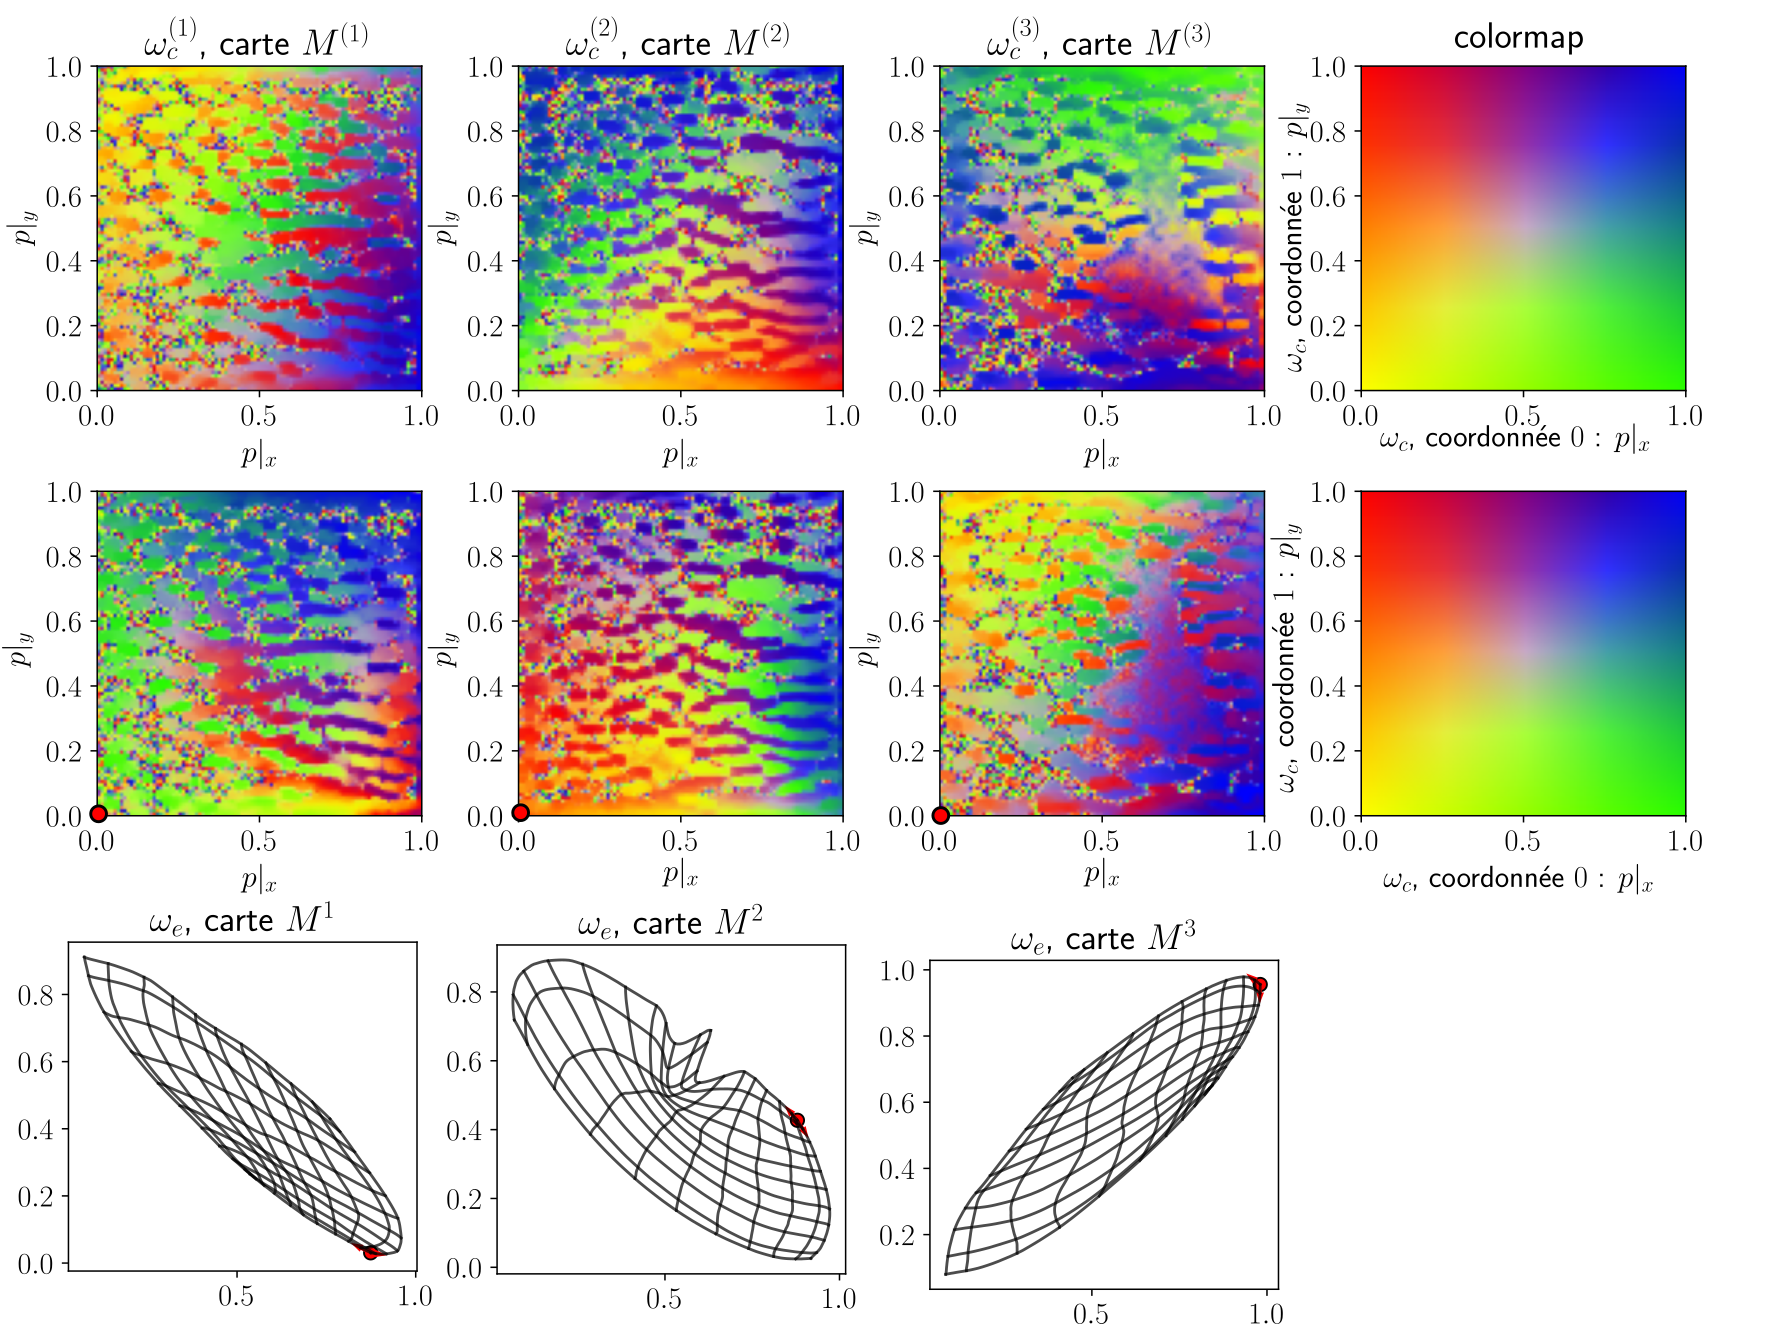
\includegraphics[width=\textwidth]{3SOM_S_wc_239999.png}
		\caption{Tracés des poids externes dans l'espace des entrées (en bas) et des deux couches de poids contextuels de chaque carte sous forme de carte de coloration. L'angle $0,0$ d'une carte est marqué par le point rouge. Les motifs formés par les poids contextuels sont similaires à ceux observés sur deux cartes. \label{fig:3som_w}}
\end{figure}

\begin{figure}
\centering\includegraphics[width=0.8\textwidth]{3SOM_error_closed.pdf}
\caption{Tracé de l'erreur de prédiction $\w_e\m{2}(\bmu\m{2})$ en fonction de la valeur théorique de $X^{(2)}$, non présentée à l'architecture, dans une architecture de trois cartes 2D prenant des entrées $X^{(i)}$ en deux dimensions $[X^{(i)}|_x, X^{(i)}|_y]$. Nous traçons sur une ligne, pour chaque entrée, les dépendances entre chacune des dimensions
lorsque la carte $M^{(2)}$ ne reçoit pas d'entrée externe. Les cartes $M^{(1)}$ et $M^{(3)}$ ayant une activité externe, le graphique montre que la quantification vectorielle est bien réalisée dans ces cartes. La carte $M^{(2)}$ est uniquement activée par les connexions contextuelles venant de $M^{(1)}$ et $M^{(3)}$. La figure centrale montre que la prédiction est correctement réalisée, mais que l'erreur de prédiction est élevée. \label{fig:3som_pred}}
\end{figure}


\section{Conclusion}

Les expériences proposées dans ce chapitre sur les cartes en deux dimensions donnent une idée des comportements auxquels on peut s'attendre dans un cas plus général d'architecture.
Ces expériences nous ont également permis d'utiliser la méthode d'étude de carte proposée tout au long de cette thèse et constituent une première application des indicateurs proposés au chapitre précédent.


Nous avons d'abord observé que l'émergence de zones de poids contextuels est une propriété qui se transpose bien sur des cartes en deux dimensions. Ces zones constituent donc un point clé des architectures CxSOM.
La formation de ces zones permet, comme sur des cartes 1D, de séparer les valeurs de $U$ en fonction des positions des BMUs et $U$ est une fonction du BMU dans chacune des cartes en deux dimensions également.
Cette séparation est correctement évaluée par le ratio de corrélation.
Nous avons observé que comme sur les cartes 1D, les zones dépendent du rapport entre les rayons de voisinage externes et contextuels et ne se forment qu'à partir d'une certaine valeur pour ce rapport.
Comme en 1D, la relaxation converge en fin d'apprentissage et le BMU 2D a donc un sens dans une carte, ce que nous avions également observé au chapitre \ref{chap:relax} pour des cartes 1D apprenant sur des entrées 1D.
Enfin, nous avons observé une bonne capacité de prédiction d'une modalité manquante sur une disposition d'entrée en sphère dans un espace 6D.

Une architecture de cartes en deux dimensions présente donc des propriétés similaires à celles observées sur les cartes 1D et généralise le comportement observé en 1D.
Cette généralisation est soumise à quelques contraintes supplémentaires aux cartes 1D.
La convergence des poids, contrairement aux cartes en une dimension, n'est pas assurée pour tous paramètres d'apprentissage et constitue un point à vérifier lors de la construction d'architectures de cartes en deux dimensions.
Par ailleurs, nous avons déplié les poids externes lors d'une étape d'initialisation afin de s'assurer que la carte 2D ne présente pas de "point de torsion". La robustesse de l'algorithme CxSOM, en particulier de la relaxation, sur des cartes "mal dépliées" peut constituer un point d'étude pour une éventuelle application de l'algorithme.
Enfin, dans le cas ou les entrées sont indépendantes, dans lequel une même position de BMU pour $M\m{1}$ correspond à toutes les positions de BMUs $[0,1]^2$ pour $M\m{2}$, les poids contextuels ne se déplient pas localement de façon à cartographier tout l'espace $[0,1]^2$.
Ce comportement se rapproche du cas limite observé sur les architectures de 10 cartes 1D. 
Les cartes 2D ont ainsi le même comportement que les cartes 1D lorsque les entrées sont indépendantes~: les poids contextuels se moyennent autour d'une position centrale et l'activité liée à ces poids contextuels n'intervient alors plus dans le calcul de l'activité globale.
Ce comportement apparaît comme une capacité de l'architecture à détecter automatiquement les relations entre entrées. Cependant, il peut aussi être un facteur limitant l'apprentissage d'entrées lorsque le modèle $U$ est de grande dimension, marquant une trop grande rigidité des poids contextuels. 

Le passage de 1D à 2D apporte également une diversité dans les comportements d'apprentissage observés en 1D: la forme des motifs spatiaux formés par les poids contextuels est plus variable que dans le cas des cartes en une dimension.
Cela peut être un atout pour le modèle, car cela laisse la porte ouverte à des comportements plus complexes sur des grandes architectures cartes 2D~; mais cela nécessite plus d'outils pour une compréhension des mécanismes d'apprentissage.
Ainsi, il sera pertinent d'étudier le comportement d'une architecture de cartes d'un point de vue macroscopique pour la suite des travaux, à partir d'indicateurs et de représentations portant sur la réponse globale d'une architecture, et non seulement à l'échelle d'une carte comme nous l'avons fait dans cette thèse.



\ifSubfilesClassLoaded{
    \printbibliography
    %\externaldocument{../main.tex}   
}{}
\end{document}



% PLAN


% Convergence des poids :
% - Dépend des paramètres, contrairement à la carte en 1D on n'arrive pas forcément dans une position stable
% - Rc = 0.02 : point fixe, avec une partie 
% - Chaque expérience différente : grande dépendance aux conditions initiales. 